\documentclass[8pt,twoside]{extarticle}
\usepackage[english]{babel}
\usepackage[utf8]{inputenc}
\usepackage{xcolor}

% for printing
%\usepackage[a4paper,inner=2.3cm,outer=1.2cm,top=2cm,bottom=2cm, asymmetric, twoside]{geometry}
\usepackage[a4paper,inner=1.75cm,outer=1.75cm,top=2cm,bottom=2cm, asymmetric, twoside]{geometry} 
%\usepackage{blindtext}
\usepackage{setspace}
%\usepackage{float}
\usepackage{titletoc}
\usepackage{titlesec}
%\usepackage{wrapfig}
%\usepackage{tikz}
\usepackage{amsmath} 
\usepackage{multicol}
\usepackage{amsfonts} 
\usepackage{comment}
%\usepackage{booktabs}
\usepackage{bbm}
%\usepackage{wrapfig}
%\usepackage{verbatimbox}
\usepackage{enumitem}
\usepackage{framed}
\usepackage[framemethod=TikZ]{mdframed}
%\usepackage{bigints}
\onehalfspacing
\usepackage[hidelinks]{hyperref}
\usepackage[round, sectionbib]{natbib} 
\usepackage{tcolorbox}

%\usepackage{titlesec}
\newcommand{\sectionbreak}{\clearpage}

\setcounter{tocdepth}{4}
\titleformat*{\paragraph}{\large\bfseries}

\usepackage{tikz}
\usepackage{adjustbox}


\setlength{\parindent}{0pt}
\renewcommand{\indent}{\hspace*{15pt}}


%\allowdisplaybreaks

\setlength\parindent{0pt}
\setlength{\parskip}{0pt}

\newcommand{\zerodisplayskips}{%
  \setlength{\abovedisplayskip}{2pt}%
  \setlength{\belowdisplayskip}{2pt}%
  \setlength{\abovedisplayshortskip}{2pt}%
  \setlength{\belowdisplayshortskip}{2pt}}
\appto{\normalsize}{\zerodisplayskips}
\appto{\small}{\zerodisplayskips}
\appto{\footnotesize}{\zerodisplayskips}

\newcommand\independent{\protect\mathpalette{\protect\independenT}{\perp}}
\def\independenT#1#2{\mathrel{\rlap{$#1#2$}\mkern2mu{#1#2}}}
\newcommand{\indep}{\perp \!\!\! \perp}
\newcommand{\compi}{\mathrm{i}\mkern1mu}




% Inhaltsverzeichnis mit zwei Spalten
%\usepackage[toc]{multitoc}
%\renewcommand*{\multicolumntoc}{2}
%\renewcommand\contentsname{}
\makeatletter
\renewcommand\tableofcontents{%
    \@starttoc{toc}%
}
\makeatother
\newcommand*{\setupTOC}{%
\titleformat{\chapter}{}{}{0pt}{} 

\titlespacing*{\chapter}{0pt}
{*7} %  % vertical space before the title <<<<<<<<<<
{*-15}  %  idem after title (in ex units + glue) <<<<<<<<<<<
}




%Überschriftengrößen anpassen, so dass Paragraph kleiner ist als Subsubsection
\titleformat{\section}
  {\normalfont\fontsize{16}{15}\bfseries}{\thesection}{1em}{}
\titleformat{\subsection}
  {\normalfont\fontsize{14}{15}\bfseries}{\thesubsection}{1em}{}
\titleformat{\subsubsection}
  {\normalfont\fontsize{12}{15}\bfseries}{\thesubsubsection}{1em}{}


\begin{document}

%\topskip0pt
\vspace*{18em}

\hrule
\begin{center}
{\fontsize{30}{60}\selectfont \textbf{Causal Inference}} \\ \

{\fontsize{20}{60}\selectfont a summary}
\end{center}
\hrule


% Table of Contents
\newpage
 
{\Huge \bfseries Table of Contents \bigskip}    

\begin{multicols}{2}
{\setupTOC  \tableofcontents}
\end{multicols}



% weitere Anpassungen im Hauptteil des Dokuments
\raggedright %linksbündig
\setlength{\columnseprule}{0.3pt} %Liniendicke zwischen zwei Multicols


%-------------------------------------------------------------------------------

% SECTION: PREREQUISITES

%-------------------------------------------------------------------------------

% this is what Introduction to Modern Causal Inference (Schuler, van der Laan) suggests
\section{Prerequisites}

% intro to real analysis
\subsection[Real Analysis]{Real Analysis \citep{abbott2015understanding}}

\begin{multicols}{2}


\paragraph{Real Numbers}  \textit{triangle inequality} $|a+b| \leq |a| + |b|$

 \textit{Density of Q in R:} $\forall a,b\in\mathbb{R}: \exists r\in \mathbb{Q}: a<r<b$

 \textit{Archimedian Property:} $\forall x {\in} \mathbb{R}\, \exists n{\in}\mathbb{N}: x<n$ \& $\forall y{>}0 \, \exists n{\in}\mathbb{N}: \frac{1}{n}{<}y$


 \textbf{Bounds of $A\subseteq \mathbb{R}$} upper: $\exists b\in \mathbb{R}$ s.t.\ $a\leq b$ $\forall a\in A$ (lower: $\geq$)

 \textit{least upper bound (supremum)} $s \in \mathbb{R}$ s.t.\ $s$ is upper bound \& $\forall$ upper bounds $b$: $s\leq b$; greatest lower (infimum) analogous


 \textbf{Cardinality:} $A\sim B$, if $\exists f:A\to B$, where $f$ bijective (in+sur)

 \textit{function} $f:A\to B$ mapping $f(x)=...$, domain = $A$, range $\subseteq B$
\textit{in/1-1:} $a_1{\neq} a_2 \Rightarrow f(a_1){\neq} f(a_2)$;
\textit{sur/onto:} if $\forall b{\in} B \, \exists a{\in} A: f(a){=}b$


 \textbf{Axiom of Completeness:} every nonempty set of real numbers that is bounded above has a least upper bound; AoC, NIP, BW, CC, MCT are equivalent: if one is assumed the others follow



 \textbf{Nested Interval Property:} if $I_n {=}\left[a_n,b_n\right]{=}\left\{x{\in}\mathbb{R}\!:a_n{\leq} x {\leq} b_n\right\}$, where $n\in \mathbb{N}$ and $I_1\supseteq I_2 \supseteq I_3 ...$, then $\cap_{n=1}^\infty I_n \neq \emptyset$



\paragraph{Sequences} are functions with domain $\mathbb{N}$

 \textbf{Convergence:} $(a_n)$ converges to $a\in\mathbb{R}$ if $\forall \epsilon>0\exists N \in\mathbb{N}$ s.t.\ $n\geq N \Rightarrow |a_n-a|<\epsilon$; written as $\lim a_n = a$ or $(a_n)\to a$

 \textit{Cauchy Criterion:} sequence converges $\Leftrightarrow$ is Cauchy sequence

 \textit{Cauchy sequence:} $\forall \epsilon>0\exists N\in\mathbb{N}$ s.t.\ $m,n\geq N\Rightarrow |a_n-a_m|<\epsilon$

 \textbf{Boundedness:} $(x_n)$ is bounded if $\exists M>0$ s.t.\ $|x_n|\leq M \,\forall n\in \mathbb{N}$

 \textbf{Algebraic Limit Theorem:} if $(a_n){\to} a$, $(b_n){\to} b$, then $(ca_n) {\to} ca$, $(a_n {+} b_n){\to} a{+}b$, $(a_nb_n){\to} ab$, $(a_n/b_n){\to} a/b$ for $b\neq 0$

 \textbf{Order Limit Theorem:} $a_n\geq 0 \, \forall n\in\mathbb{N} \Rightarrow a\geq 0$ ($\leq$ analogous), $\exists c\in\mathbb{R}$ s.t.\ $c\leq b_n\forall n\in\mathbb{N}\Rightarrow c\leq b$ ($\geq$ analogous)



 \textbf{Monotone Convergence Theorem:} bounded \& monotone (\textit{increasing} $a_n {\leq} a_{n+1}$ or \textit{decreasing} $a_n {\geq} a_{n+1}$) sequences converge



 \textbf{Bolzano-Weierstrass Theorem:} 
 
 all bounded sequences have a convergent subsequence

 \textit{subsequences} of a convergent sequence converge to the same limit




\paragraph{Series} infinite series are sums over sequences: $\sum_{n=1}^\infty b_n$

 \textit{harmonic series} $\sum_{n=1}^\infty \frac{1}{n}$
, \textit{geometric series} $\sum_{k=0}^\infty ar^k \overset{|r|<1}{=} \frac{a}{1-r}$

 \textbf{Convergence:} to $B$, if $(s_m){\to} B$, partial sums $s_m=\sum_{n=1}^m b_n$

 \textit{Cauchy Criterion:} $\sum_{k=1}^\infty a_k$ converges $\Leftrightarrow$ \newline
$\forall \epsilon>0\exists N\in\mathbb{N}$ s.t.\ $n>m\geq N \Rightarrow |a_{m+1} + a_{m+2}+...+a_n|<\epsilon$;
that implies if $\sum_{k=1}^\infty a_k$ converges then $(a_k)\to 0$



 \textbf{Algebraic Limit Theorem:}  if $\sum_{k=1}^\infty a_k = A$ and $\sum_{k=1}^\infty b_k = B$ then $\sum_{k=1}^\infty ca_k = cA$ and $\sum_{k=1}^\infty a_k+ b_k = A+B$


 \textbf{Cauchy Condensation Test:} if $(b_n)$ is decreasing and $b_n\geq 0\forall n\in \mathbb{N}$ then: $\sum_{n=}^\infty b_n$ converges $\Leftrightarrow \sum_{n=0}^\infty 2^nb_{2^n}$ converges


 \textbf{Comparison Test:} if $0\leq a_k \leq b_k \forall k\in \mathbb{N}$, then $\sum_{k=1}^\infty b_k$ converges $\Rightarrow \sum_{k=1}^\infty a_k$ too \& $\sum_{k=1}^\infty a_k$ diverges $\Rightarrow \sum_{k=1}^\infty b_k$ too

 \textbf{Absolute Convergence Test:} 
$\sum_{n=1}^\infty |a_n|$ conv $\Rightarrow$ $\sum_{n=1}^\infty a_n$ too

 \textbf{Alternating Series Test:} if $(a_n)$ is decreasing and converges, then $\sum_{n=1}^\infty (-1)^{n+1}a_n$ converges

 \textbf{Absolute Convergence:} if $\sum_{n=1}^\infty |a_n|$ converges then $\sum_{n=1}^\infty a_n$ converges \textit{absolutely}, if only the latter, then \textit{conditionally}

 \textbf{Rearrangements:} if $\sum_{k=1}^\infty a_k$ converges absolutely, then any rearrangement converges to the same limit

 \textbf{Double Series:} if $\sum_{i=1}^\infty\sum_{j=1}^\infty |a_{ij}|$ converges 
$\Rightarrow \sum_{i=1}^\infty\sum_{i=1}^\infty a_{ij} $ 
$= \sum_{j=1}^\infty\sum_{i=1}^\infty a_{ij} = \lim_{n\to\infty} s_{nn}$, 
where $s_{nn} = \sum_{i=1}^n\sum_{j=1}^n a_{ij}$


\paragraph{Sets}

 \textit{Cantor Set:} $C=\cap_{n=0}^\infty C_n$, with $C_n$ removing the middle third of all intervals, e.g.\ $C_1 = C_0\setminus(\frac{1}{3}, \frac{2}{3})=\left[0,\frac{1}{3}\right]\cup \left[\frac{2}{3},1\right]$

 \textbf{Open Sets:} $\forall a\in O\,\exists V_\epsilon(a)\subseteq O$,
 with $\epsilon$-neighborhood of $a$ $V_\epsilon(a)=\left\{x\in\mathbb{R}:|x-a|<\epsilon\right\}$; union of open sets is open, the finite intersecton of open sets is open
 
  \textbf{Closed Sets:} contain their limit points $\Leftrightarrow$ every Cauchy sequence has a limit that lies within the set \newline
 $x$ is \textit{limit point} of $A$ $\Leftrightarrow \forall \epsilon>0 \, V_\epsilon(x)\cap A$ includes other points than $x$ $\Leftrightarrow$ $x=\lim(a_n)$ for some $(a_n)\in A$ with $a_n\neq x \forall n\in \mathbb{N}$; \newline
  all non limit point $a\in A$ are \textit{isolated points}; the finite union of closed sets is closed, the intersection of closed sets is closed
  
   \textbf{Closure:} $\bar{A}=A\cup L$, with $L$ the set of $A$'s limit points; the closure is the smallest closed set containing $A$
  
   \textbf{Complement:} $A^c = \left\{x\in\mathbb{R}:x\notin A\right\}$; 
  $A$ closed $\Leftrightarrow$ $A^c$ open
  
  
   \textbf{Compact $\Leftrightarrow$ Bounded and Closed $\Leftrightarrow$ $\exists$ Finite Subcover}
  
  \begin{itemize}[itemsep=0em, topsep=0pt, partopsep=0pt,parsep=0pt, leftmargin=1.5em]
  \item \textit{Compactness:} $K$ compact $\Leftrightarrow$ every sequence has a subsequence that converges in $K$; the intersection of a sequence of nested nonempty compact sets is not empty
  \item \textit{Boundedness:} $\exists M>0$ s.t.\ $|a|\leq M \,\forall a\in A$
\item\textit{Any open cover for $A$ has a finite subcover:} An open cover is a set of open sets $\left\{O_\lambda:\lambda\in\Lambda\right\}$ whose union contains $A$; a finite subcover is a finite subset that still covers $A$
  \end{itemize}
  
 \textbf{Perfection:} closed and no isolated points; a nonempty perfect set is uncountable; the Cantor set is perfect

 \textbf{Separation:} of $A$ and $B$ if $\bar{A}\cap B =\emptyset$ \& $A\cap \bar{B}=\emptyset$

 \textbf{Disconnection:} if $A=B\cup C$, with $B,C$ nonempty \& separated;
\newline
$E$ is \textit{connected} $\Leftrightarrow$ all nonempty disjoint sets  $B,C$ s.t.\ $E=B\cup C$ have a convergent sequence with a limit in the other set $\Leftrightarrow$ whenever $a<c<b$ with $a,b\in E$, then $c \in E$

  \textbf{Baire's Theorem:} $\mathbb{R}$ cannot be written as the countable union of nowhere-dense sets; $E$ is \textit{nowhere-dense} if $\bar{E}$ contains no nonempty open intervals

\paragraph{Functional Limits and Continuity}  \ \\

 \textbf{Functional Limit:} let $f:A\to\mathbb{R}$ and $c$ limit point of $A$
if $\forall \epsilon > 0 \, \exists \delta>0$ s.t.\ $0<|x-c|<\delta$ (and $x\in A$) it follows $|f(x)-L|<\epsilon$, then $\lim_{x\to c} f(x)=L$

 \textit{Sequential Criterion:}  $\lim_{x\to c} f(x)=L \Leftrightarrow$ for all sequences $(x_n)\subseteq A$, with $x\neq c$ and $(x_n)\to c$ follows $f(x_n)\to L$

 \textbf{Algebraic Limit Theorem:} if $\displaystyle\lim_{x\to c}f(x)=L$ and $\displaystyle\lim_{x\to c}g(x)=M$ then \,\,\,
$\displaystyle\lim_{x\to c}kf(x)=kL$;  \,\,\,
$\displaystyle\lim_{x\to c}\left[f(x) + g(x)\right]=L+M$; $\displaystyle\lim_{x\to c}\left[f(x)g(x)\displaystyle\right]=LM$; \,\,\, $\displaystyle\lim_{x\to c}f(x)/g(x)=L/M$ if $M\neq 0$

 \textbf{Divergence Criterion:} if $(x_n)$ and $(y_n)$ with $x_n\neq c \neq y_n$ and $\lim x_n{=}\lim y_n{=}c$ but $\lim f(x_n) {\neq} f(y_n)$ then $\not\!\exists$ $\lim_{x\to c}f(c)$ 

 \textbf{Continuity at $\boldsymbol{c}$:} $\forall \epsilon>0\,\exists \delta>0$ s.t.\ whenever
 $|x-c|<\delta$ (and $x\in A$) then $|f(x)-f(c)|<\epsilon$, 
 can also be expressed as: \newline $(x_n)\to c$ (with $x_n \in A$) $\Rightarrow f(x_n)\to f(c)$
 
  \textbf{Algebraic Continuity Theorem:} if $f,g$ continuous at $c$ then these are too: $kf(x)$, $f(x){+}g(x)$, $f(x)g(x)$, $f(x)/g(x)$ (if $g(x){\neq} 0$)
 
  \textbf{Compositions:} $f$  continuous at $c$ and $g$ is continuous at $f(c)$ $\Rightarrow g\circ f$ is continuous at $c$ (if $g \circ f(x)$ well-defined)
 
  \textbf{Boundedness:} $f$ is bounded on its domain $A$ $\Leftrightarrow$ $f(A)$ is bounded; $f$ is bounded \textit{on $B\subseteq A$} $\Leftrightarrow$ $f(B)$ is bounded

 \textbf{Preservation of Compact Sets:} $K$ compact $\Rightarrow$ $f(K)$ is too;
if $f$ is continuous on a compact set, $f$ attains min/max values

 \textbf{Uniform Continuity:} $\forall \epsilon>0\,\exists \delta>0$ s.t.\ whenever
 $|x-y|<\delta$ then $|f(x)-f(y)|<\epsilon$ (i.e.\ difference between them is bounded);
 $f$ continuous on compact set $K$ $\Rightarrow$ $f$ uniformly continuous on $K$
 
  \textit{Sequential Criterion for Nonuniformity:} $\exists \epsilon_0>0$ and $(x_n),(y_n)$ in $A$ s.t.\ $|x_n-y_n|\to 0$ but $|f(x_n) - f(y_n)|>\epsilon_0$


 \textbf{Intermediate Value Theorem:} $f:[a,b]\to\mathbb{R}$ continuous then $f(a)<L<f(b)$ $\Rightarrow$ $\exists c\in (a,b)$, where $f(c)=L$

 alternatively: \textit{Preservation of Connectedness:} $f:A\to \mathbb{R}$ continuous, $E\subseteq A$ connected $\Rightarrow$ $f(E)$ connected

 \textit{Intermediate Value Property} (converse of IVM): $f$ has IVP on $\left[a,b\right]$ if $\forall x<y$ \& $L$ s.t.\ $f(x)<L<f(y)$ $\exists c\in(x,y)$, where $f(c)=L$ (implies continuity if $f$ is monotone)
 
 \textbf{Discontinuity:} 
 
 \vspace{-1.4em}
 \begin{itemize}[itemsep=0em, topsep=0pt, partopsep=0pt,parsep=0pt, leftmargin=8.5em]
 \item \textit{removable}: if $\lim_{x\to c}f(x)$ exists but $\neq f(c)$
 \item \textit{jump}: $\lim_{x\to c^+}f(x) \neq \lim_{x\to c^-}f(x)$ 
 \item \textit{essential}: not continuous for another reason
 \end{itemize}
 
 \textbf{The Set of Discontinuous Points} $D_f$  can be written as the countable union of closed sets ($ =: F_\sigma$)



\paragraph{Derivation} $g'(c)=\lim_{x\to c} \frac{g(x)-g(c)}{x-c}$ \newline
$(f{+}g)'(c) = f'(c) {+} g'(c)$; \,\,\, $(fg)'(c)=f'(c)g(c) {+} f(c)g'(c)$; $(kf)'(c) = kf'(c)$; \,\,\, $(f/g)'(c) =\frac{g(c)f'(c)-f(c)g'(c)}{g^2(c)}$, for $g(c)\neq 0$; 
$(g\circ f)'(c)=g'(f(c))\cdot f'(c)$


\textbf{Differentiability:} Differentiability at $c$ implies continuity at $c$

\textbf{Interior Extremum Theorem:} let $f$ differentiable on $(a,b)$; if $f$ has a maximum or minimum at $f(c)$, then $f'(c)=0$


\textbf{Darboux's Theorem:} if $f$ differentiable on $\left[a,b\right]$ and $f'(a)<\alpha<f'(b)$ then $\exists c\in (a,b)$, where $f'(c)=\alpha$


\textbf{Rolle's Theorem:} $f(a)=f(b) \Rightarrow \exists c\in (a,b)$ with $f'(c)=0$

\textbf{Mean Value Theorem:} if $f:[a,b]\to\mathbb{R}$ continuous on $[a,b]$ and differentiable on $(a,b)$ then $\exists c\in(a,b)$ with $f'(c)=\frac{f(b)-f(a)}{b-a}$

\textbf{Generalized Mean Value Theorem:} $f,g$ continuous on $[a,b]$ and differentiable on 
$(a,b)$ $\Rightarrow \exists c\in(a,b)$ with $\left[f(b)-f(a)\right]g'(c) = $  $ \left[g(b)-g(a)\right]f'(c)$; 
if $g\neq0$: $\frac{f'(c)}{g'(c)}=\frac{f(b)-f(a)}{g(b)-g(a)}$

\textbf{L'Hopital's Rules:} 

\textbf{0/0: } let $a\in I$, $f,g$ continuous on $I$, differentiable on $I\setminus a$:  

if $f(a){=}0{=}g(a)$ then $\lim_{x\to a}\frac{f'(x)}{g'(x)} = L \Rightarrow \lim_{x\to a}\frac{f(x)}{g(x)} = L$

\textbf{$\boldsymbol{\infty}$/$\boldsymbol{\infty}$: } let $f,g$ differentiable on $(a,b)$:

if $\lim_{x\to a}g(x)=\infty$ then $\lim_{x\to a}\frac{f'(x)}{g'(x)}=L \Rightarrow \lim_{x\to a}\frac{f(x)}{g(x)}=L$

\ \\


\paragraph{Functional Sequences} \ \\

\textbf{Convergence:} let $f_n$ be defined on $A\subseteq\mathbb{R}$ 

\textit{Pointwise:} if  $\lim_{n\to \infty} f_n(x)=f(x)$ $\forall x \in A$ then $f_n\to f$

\textit{Uniform:} $\forall \epsilon>0 \,\exists N\in\mathbb{N}$ s.t.\ $|f_n(x)-f(x)|<\epsilon \,\,\, \forall x\in A, n\geq N$

\textit{Cauchy Criterion:} $(f_n)$ converges uniformly if and only if  $\forall \epsilon > 0\,\exists N\in \mathbb{N}$ s.t.\ $|f_n(x)-f_m(x)|<\epsilon  \,\,\, \forall x\in A, m,n \geq N$

\textbf{Continuity:}  let $(f_n)$ converge uniformly to $f$, if all $f_n$ are continuous at $c\in A$, then $f$ is in continuous at $c$

\textbf{Differentiability:} let $(f_n)$ differentiable on $[a,b]$ and $(f'_n) \to g$ uniformly on $[a,b]$; if $\exists x_0\in[a,b]$ where $f_n(x_0)$ convergent, then (1) $(f_n)$ converges uniformly (2) $f{=}\lim f_n$ differentiable (3) $f'{=}g$

\paragraph{Functional Series} $\sum_{n=1}^\infty f_n(x)$

\textbf{Convergence:} converges \textit{pointwise (uniformly)} on $A$ to $f(x)$ if sequence of partial sums converges pointwise (uniformly) to $f(x)$

\textit{Cauchy Criterion:} $\forall \epsilon>0 \,\exists N\in \mathbb{N}$ s.t.\ $\forall n>m\geq N: |f_{m+1}(x) + f_{m+2}(x) + ... f_{n}(x)| <\epsilon \,\forall x\in A$

 \textit{Weierstrass M-Test:} let $(f_n)$ defined on $A\subseteq \mathbb{R}$, let $M_n>0$ satisfy $|f_n(x)|\leq M_n \,\forall x\in A$; if $\sum_{n=1}^\infty M_n$ converges, then $\sum_{n=1}^\infty f_n$ converges uniformly on $A$
 
 \textbf{Power Series:} $f(x)=\sum_{n=0}^\infty a_nx^n$

\textit{Convergence:} $f(x)$ converges for $x_0\in \mathbb{R}$ $\Rightarrow$ converges absolutely for any $x$ with $|x|\leq |x_0|$ (the set of convergence is $(/[-R,R]/)$ with $R\in\mathbb{R}_0^+ \cup \infty$, $R$ is called the radius of convergence)

\textit{Abel's Theorem:} let $f(x)$ converges at $x=R>0$; then $f(x)$ converges uniformly on $[0,R]$ (similar for $x=-R$);

\textit{Uniform Convergence:} if a power series converges pointwise on $A\subseteq \mathbb{R}$, then it converges uniformly on any compact set $K\subseteq A$


\textit{Differentiability:} if $f(x)$ converges on interval $A\subseteq \mathbb{R}$, then

\begin{itemize}[itemsep=0em, topsep=0pt, partopsep=0pt,parsep=0pt, leftmargin=1.0em]
\item $f$ continuous on $A$ and differentiable on any $(-R,R)\subseteq A$
\item the derivative is $f'(x)=\sum_{n=1}^\infty na_nx^{n-1}$
\item $f$ is infinitely differentiable on $(-R,R)$ 
\end{itemize} 

\textbf{Taylor Series:}  $f(x)=\frac{f^{(n)}(a)}{n!} (x-a)^n$ \,\,\,(here $a=0$)

\textit{Lagrange's Remainder Theorem:} let $f$ infinitely differentiable on $(-R,R)$, define $a_n=f^{(n)}(0)/n!$, let $S_N$ partial sums to $N$, then for $x\neq 0$ $\exists c:|c|{<}|x|$, where error $f(x){-}S_N(x)=\frac{f^{(N+1)}(c)}{(N+1)!}x^{N+1}$



\end{multicols}

%\newpage

% measure theoretic probability
\subsection[Measure Theory]{Measure Theory \citep{capinski_measure_2004}}

\begin{multicols}{2}


\paragraph{Riemann Integral} coinciding upper $U$ and lower $L$ sums

for partitions $P$: $U=\sum_{i=1}^n \sup_{p_i} \mathrm{len}(p_i)$; $L=\sum_{i=1}^n \inf_{p_i} \mathrm{len}(p_i)$

\textbf{Riemann's Criterion:} $f$ integrable iff $\forall \epsilon> 0 \,\exists P_\epsilon$ s.t.\ $U{-}L <\epsilon$

\textbf{Fundamental Theorem of Calculus:} if $f:[a,b]\to \mathbb{R}$ continuous and $F'=f$, then $F(b)-F(a)=\int_a^bf(x)\mathrm{d} x$

\textbf{Problems:} why do we need a Lebesgue integral?
\begin{itemize}[itemsep=0em, topsep=0pt, partopsep=0pt,parsep=0pt, leftmargin=1.0em]
\item scope: many results need continuous $f$ and bounded intervals
\item dependence on intervals: otherwise often not defined
\item lack of completeness: $\int_a^b f_n(x) \mathrm{d}x \to \int_a^b f(x) \mathrm{d}x$ doesn't hold
\end{itemize} 

\paragraph{Measure} $\mathcal{B}\subset\mathcal{M}\subset\mathcal{P}(\mathbb{R})$

\textbf{Null Sets} $\forall \epsilon>0 \,\exists$ a sequence of intervals $(I_n)$ s.t.\ \newline $A\subseteq \bigcup_{n=1}^\infty I_n$ and $\sum_{n=1}^\infty l(I_n)<\epsilon$ ($=\exists$ arbitrarily small cover);

the union of a sequence of null sets is also null

\textbf{Lebesgue Outer Measure} of $A$: $m^*(A)=\inf Z_A$, with 
$Z_A = \left\{ \sum_{n=1}^\infty l(I_n): I_n \text{ are intervals, } A\subseteq \bigcup_{n=1}^\infty I_n \right\}$

\begin{itemize}[itemsep=0em, topsep=0pt, partopsep=0pt,parsep=0pt, leftmargin=1.0em]
\item null sets have outer measure zero
\item monotonicity: $A\subset B \Rightarrow m^*(A)\leq m^*(B)$
\item the outer measure of an interval equals its length
\item countable subadditivity: $m^*\left(\bigcup_{n=1}^\infty E_n\right)\leq \sum_{n=1}^\infty m^*(E_n)$
\item translation invariance: $m^*(A)=m^*(A+t)$
\end{itemize}

\textbf{Lebesgue Measurability:} of $E\subseteq\mathbb{R}$ (write $E\in\mathcal{M}$) if $\forall A\subseteq \mathbb{R}: m^*(A)=m^*(A\cap E)+m^*(A\cap E^c)$ (additivity)

\textit{$\mathcal{M}$ is a $\sigma$-field:} and countably additive ($=:$ measure)

\begin{itemize}[itemsep=0em, topsep=0pt, partopsep=0pt,parsep=0pt, leftmargin=1.0em]
\item $\mathbb{R}\in \mathcal{M}$ (btw so are all null sets and intervals)
\item $E\in\mathcal{M}\Rightarrow E^c\in \mathcal{M}$
\item $E_n{\in} \mathcal{M}\,\forall n \Rightarrow \bigcup_{n=1}^\infty E_n \in \mathcal{M}$, with countable additivity: $m^*(\bigcup_{n=1}^\infty E_n) = \sum_{n=1}^\infty m^*(E_n)$ for $E_j\cap E_k=\emptyset$ if $j\neq k$
\end{itemize}
(it follows that $\mathcal{M}$ is closed under countable intersections as well)
the intersection of $\sigma$-fields is a $\sigma$-fields

\textit{Open Sets:} every open set in $\mathbb{R}$ can be expressed as a union of countable open intervals $\Rightarrow$ all open sets are in $\mathcal{M}$

\textbf{Lebesgue Measure $m$:} $f:\mathcal{M}\to [0,\infty]$, countably additive $m^*$




\begin{itemize}[itemsep=0em, topsep=0pt, partopsep=0pt,parsep=0pt, leftmargin=1.0em]
\item let $A_n\in \mathcal{M}: A_n\subset A_{n+1} \forall n \Rightarrow m(\bigcup_n A_n)=\displaystyle\lim_{n\to \infty} m(A_n)$ \newline
\hspace{1em} let $m(A_n)<\infty: A_n\supset A_{n+1} \forall n \Rightarrow m(\bigcap_n A_n)=\displaystyle\lim_{n\to \infty} m(A_n)$
\item $m$ is continuous at $\emptyset$, i.e.\ $(B_n)$ decrease to $\emptyset$ $\Rightarrow m(B_n)\to 0$
\end{itemize}









\textbf{Borel Sets:} $\sigma$-field generated by a family of sets
$$\mathcal{B} =\bigcap \left\{\mathcal{F}:\mathcal{F} \text{ is a } \sigma\text{-field containing all intervals}\right\}$$
$\mathcal{B}$ is also generated by intervals of a particular type

\textit{Completion:} not all null sets are in $\mathcal{B}$ \newline
$\mathcal{M}$ is the completion of $\mathcal{B}$: a measure space $(X,\mathcal{F},\mu)$ is complete if $\forall F\in\mathcal{F}$ with $\mu(F)=0$: $N\subset F$ is in $\mathcal{F}$ and $\mu(N)=0$

\textbf{Borel Regular Measure:} $\mu(B)=\inf\{\mu(O): O \text{ open}, O\supset B\}{=}$ $\sup\{\mu(F): F \text{ closed}, F \supset B\}$;
\textit{Approximations:} of $m$ for $E\in \mathcal{M}$

\textit{above:}  
$\forall \epsilon>0\,\exists$ open set $O$ s.t.\ $A\subset O,$ $m(O)\leq m^*(A)+\epsilon$

\textit{below:} if $E \in \mathcal{M}$ then $\epsilon>0\, \exists$ closed set $F\subset E$ s.t.\ $m(E\setminus F)<\epsilon$
%, hence: $\exists B{\in} E$ s.t.\ $B{=}\bigcup_nF_n$, with $F_n$ closed sets and $m(E{\setminus} B){=}0$

%eventuell reicht eins von denen
%$\forall A\in \mathbb{R} \, \exists (O_n)$ s.t.\ $A\subset \bigcap_n O_n,$ $m(\bigcap_n O_n)=m^*(A)$

\textbf{Probability} restriction to $\mathcal{M}_B=\left\{A\cap B: A \in \mathcal{M}\right\}$

\textit{Probability Space:} $(\Omega, \mathcal{F}, P)$, with $\Omega$ an arbitrary set, $\mathcal{F}$ a $\sigma$-field of subsets of $\Omega$ called events, and $P$ measure on $\mathcal{F}$ s.t.\ $P(\Omega)=1$;

%\textit{Define:} $P(A|B){=}\frac{P(A\cap B)}{P(B)}$;

\textit{Independence:} 

\begin{itemize}[itemsep=0em, topsep=0pt, partopsep=0pt,parsep=0pt, leftmargin=1.0em]
\item events $E=\{A_1,... A_n\}$: $\forall K\subseteq E: P(\bigcap_K A_i)= \prod_K P(A_i)$
\item $\sigma$-fields $S=\{\mathcal{F}_1, ... \mathcal{F}_n\}$ on $(\Omega, \mathcal{F}, P)$: $\forall S_s\subseteq S: F_i \in \mathcal{F}_j \in S_s \Rightarrow P(\bigcap_{S_s} F_i)=\prod_{S_s}P(F_i)$
\end{itemize}

\paragraph{Measurable Functions} define $f$ only up to null sets (a.e.)

\textbf{Extended $\mathbb{R}$:} $\bar{\mathbb{R}} = [-\infty, \infty]$, with $0\cdot\infty=0$ and avoid $\infty{-}\infty$

\textbf{(Lebesgue) Measurability:} target range (Riemann: domain)

$E$ is measurable, $f:E\to\mathbb{R}$ is measurable if $\forall I \subseteq \mathbb{R}:$

$f^{-1}(I)\in \mathcal{M}$ (if $\in \mathcal{B}$, then Borel(-measurable) function)

\textit{Equivalences:} $f$ is measurable $\Leftrightarrow$ $\forall a: f^{-1}(x)$ is measurable \newline for $x$ in $\{(a,\infty),[a,\infty), (-\infty,a), (-\infty,a]\}$

\textit{Measurable $f$:} constant, continuous (due to open sets), monotone

\textbf{Properties:}
m'able $f:E{\to}\mathbb{R}$: vector space, i.e. $f{+}g$, $fg$ m'able

$F:\mathbb{R}\times\mathbb{R}\to \mathbb{R}$ continuous and $f,g$ m'able $\Rightarrow$ $F(f(x),g(x))$ m'able

$f^-,f^+$ m'able $\Leftrightarrow$ $f$ m'able $\Rightarrow |f|$ m'able

%$(f_n)$ m'able $\Rightarrow$ $\displaystyle\max_{n\leq k} f_n$, $\displaystyle\min_{n\leq k} f_n$, $\displaystyle\sup_{n\in N} f_n$, $\displaystyle\inf_{n\in N} f_n$, $\displaystyle\lim\sup_{n\to \infty} f_n$, $\displaystyle\lim\inf_{n\to \infty} f_n$ m'able (also min, inf, lim inf)

$(f_n)$ m'able $\Rightarrow$ $\displaystyle\max_{n\leq k} f_n$,$\displaystyle\sup_{n\in N} f_n$,$\displaystyle\lim\sup_{n{\to} \infty} f_n$ m'able (also min etc.)

$f,g: E{\to} \mathbb{R}$, $E\in \mathcal{M}$, $f$ m'able, $\{x: f(x)=g(x)\}$ null $\Rightarrow$ $g$ m'able

$(f_n)$ m'able, $f_n(x)\to f(x)$ a.e. for $x\in E$ $\Rightarrow$ $f$ m'able

\textbf{Essential Supremum:} $\mathrm{ess}\sup f:=\inf\{z:f\leq z \text{ a.e.}\}$ (also inf)


\textbf{Probability} \textit{random variable} m'able $X:\Omega \to \mathbb{R}$

\textit{$\sigma$-field gen.\ by $X$:} $X^{-1}(\mathcal{B}){=} \left\{S{\in}\mathcal{F}: S{=}X^{-1}(B) \text{ for some } B {\in} \mathcal{B}\right\}$

\textit{probability distribution:} $P_X(B) = P(X^{-1}(B))$ is count.\ add.\

\textit{Dirac measure:} $\delta_a(B) = \mathbbm{1}(a\in B)$

\textit{$X,Y$ indep.:} $\forall B,C \text{ in } \mathbb{R}:  X^{-1}(B) \indep Y^{-1}(C)$



\paragraph{Integral} over $E \in \mathcal{M}$ with measure $m$: $\int_E f \,\mathrm{d}m$

\textbf{on \textit{simple function} $\boldsymbol{\varphi}$} (range is finite set of reals $a_i>0$, with corresp.\ domain m'able $A_i$): $\int_E \varphi \,\mathrm{d}m = \sum_{i=1}^n a_i m(A_i\cap E)$

\textbf{on m'able function $\boldsymbol{f\geq 0}$:} $\int_E f \, \mathrm{d}m = \sup Y(E,f)$, where 
$Y(E,f)=\left\{ \int_E \varphi\,\mathrm{d}m:0\leq \varphi\leq f, \varphi \text{ is simple}\right\}$; $f{=}0$ a.e.\ $\Leftrightarrow \int\! f \,\mathrm{d} m$

% there where some properties, but so far the integral is not defined on all functions, so I thought I'd wait on it. It's on p. 80. also left out prop 4.5 on p 81

\textbf{Monotone Convergence Theorem} if $\{f_n\}$ $\geq 0$, m'able,  \& $f_n \to f$ then: $\lim_{n\to\infty}\int_E f_n(x)\, \mathrm{d}m = \int_E f\,\mathrm{d}m$ \\ (if limit is only a.e.\ then $E$ has to be m'able for result to hold)

\textbf{on m'able function $\boldsymbol{f}$:} $\int_E f\, \mathrm{d}m = \int_E f^+\, \mathrm{d}m - \int_E f^-\, \mathrm{d}m $

($f$ is only integrable if both components are finite)

set of all functions that are integrable over $E$ is called $\boldsymbol{\mathcal{L}^1(E)}$

\textbf{Properties:} let $f,g$ integrable, $c\in\mathbb{R}$, $A,E$ measurable then

$f\leq g \Rightarrow \int f \, \mathrm{d}m \leq \int g \, \mathrm{d}m$; 
$\int (cf) \, \mathrm{d}m = c \int_E f \, \mathrm{d}m$;
$f{+}g \text{ int'able, } \mathcal{L}^1 \text{ vector space}$; 
$\int_E (f{+}g) \, \mathrm{d}m {=} \int_E f \, \mathrm{d}m {+} \int_E g \, \mathrm{d}m$;

$\int_A f \, \mathrm{d}m \leq \int g \, \mathrm{d}m \forall A \Rightarrow f\leq g$ a.e.; int'able $f$ is finite a.e.; 

$m(A)\inf_A f \leq \int_A f \, \mathrm{d}m \leq m(A) \sup_A f$; $|\int f \, \mathrm{d}m| \leq \int |f| \, \mathrm{d}m$;

let $f\geq 0$: (1) $\int f \, \mathrm{d}m{=}0 \Rightarrow f{=}0$ a.e.\ (2) $A\to \int_A f \, \mathrm{d}m$ is  measure

\textbf{Dominated Convergence Theorem:} $(f_n)$ measurable, $|f_n|{\leq} g$ a.e.\ on $E{\in} \mathcal{M}$, $g$ $E$-int'able $\Rightarrow$  $\displaystyle\lim_{n\to\infty} \int_E f_n(x)\,\mathrm{d}m = \int_E f \,\mathrm{d}m$

\textit{Beppo-Levi:} $\sum_{n=1}^\infty \int |f_n| \,\mathrm{d}m$ finite $\Rightarrow$ $\sum_{n=1}^\infty f_n(x)$ converges a.e., is integrable and
$\int\sum_{n=1}^\infty f_n \,\mathrm{d}m = \sum_{n=0}^\infty \int f_n \,\mathrm{d}m$

\textbf{Relation to Riemann integrals:} let $[a,b] \to \mathbb{R}$ bounded

$f$ continuous a.e.\ $\Leftrightarrow$  $f$ is R-int'able $\Rightarrow$ $f$ is L-int'able ($F_R=F_L$)

L-int's also equal improper R-int's (e.g. $\displaystyle\lim_{a\to -\infty, b\to \infty} \int_a^b f(x)dx$)

\textbf{Approximating m'able functions:}

 $f$ on $[a,b]$ bounded: $\forall \epsilon>0\, \exists$ step function $h$ s.t.\ $\int_a^b|f{-}h|\,\mathrm{d}m\leq \epsilon$
 
 $f{\in} \mathcal{L}^1$: $\forall \epsilon{>}0 \, \exists g$ (cont's, zero outside int.) s.t. $\int|f{-}h|\,\mathrm{d}m\leq \epsilon$
 
 \textit{Riemann-Lebesgue:} $f{\in}\mathcal{L}^1$: $s_n {=} \int_{{-}\infty}^\infty f(x)\overset{(\cos)}{\sin} (kx)  \,\mathrm{d}x$ go to 0

\textbf{Probability:} for r.v.\ $X$: $\int_\Omega g(X(\omega))\,\mathrm{d}P(\omega) = \int_\mathbb{R} g(x)\,\mathrm{d}P_X(x)$

\textit{absolutely continuous:} int'able $f\geq 0$, where measure $A\to P(A)=\int_A f \,\mathrm{d}m$; $f$ is called a \textit{density} with $\int f \,\mathrm{d} m = 1$; 

\textit{cdf:} defined as $F(y)= P_X((-\infty, y])\overset{a.c.}{=}\int_{-\infty}^y f(x) \,\mathrm{d}x$,
 continuity of $F$ does not imply $f$ exists (see Lebesgue function), 

$F_X$ is 1 non-decreasing, 2 right continuous and 3 goes from 0 to 1,

%if $F:\mathbb{R}\to [0,1]$ fulfills 1-3: $\exists$ r.v.\ on $\mathcal{B}$ $X:[0,1]\to\mathbb{R}$, s.t.\ $F=F_X$

%let $P_X$ defined on $\mathbb{R}^n$ absolutely continuous with density $f_X$, $g:\mathbb{R}^n\to \mathbb{R}$ int'able $\Rightarrow$ $\int_{\mathbb{R}^n}g(x)\,\mathrm{d} P_X(x)=\int_{\mathbb{R}^n} f_X(x)g(x)\, \mathrm{d}x$

$g:\mathbb{R}\to\mathbb{R}$ increasing  \& diff'able: $f_{g(X)}(y){=}f_X(g^{-1}(y))\frac{\mathrm{d}}{\mathrm{d}y}g^{-1}(y)$

\textit{Expectation:} $\mathbb{E}(X)=\int_{\Omega}X\,\mathrm{d}P
=\int x\,\mathrm{d}P_X(x)
\overset{a.c.}{=}\int xf_X(x)\,\mathrm{d}x$

\textit{$\mathbb{C}$:} $\int_E u+\compi v \,\mathrm{d}m = \int_E u \,\mathrm{d}m  + \compi \int_E v \,\mathrm{d}m $, $|\int_E f \,\mathrm{d}m| \leq \int_E |f| \,\mathrm{d}m$

\textit{Characteristic Function:} $\varphi_X(t)=\mathbb{E}(\exp^{\compi tX}) = \int \exp^{\compi tx} \, \mathrm{d}P_X(x)$ for r.v.\ $X$, with $t\in \mathbb{R}$;
$\varphi_X(0)=1$, $-1\leq\varphi_X(t)\leq 1$


\paragraph{Spaces Of Integrable \textit{f}} $\infty$-dim.\ normed vector spaces 





\textbf{$\boldsymbol{L^1}$} (Banach space := complete normed space): \\ 

\textbf{\textit{norm:}} $x\to \|x\|$, with $x\in$ vector space: $\| x\|\geq 0$, $\| x\|=0 \Leftrightarrow x=0$, $\|\alpha x\| =|\alpha| \| x\|$ ($\alpha\in\mathbb{R}/\mathbb{C}$), triangle equality

\textbf{\textit{metric:}}  $d:X\times X \to \mathbb{R}$ ($X$ set), with $d(x,y)\geq 0$, symmetric, $d(x,y){=}0 \Leftrightarrow x{=}y$, triangle equality; e.g.: $d(x,y)=\|x{-}y\|$

consider vector space $L^1(E) = \mathcal{L}^1(E)/_\sim$, where $f\sim g \Leftrightarrow $ $ f(x)=g(x)$ a.e.\ with $\|f\|_1=\int_E|f|\,\mathrm{d}m$, $L^1(E)$ is complete

\textbf{$\boldsymbol{L^2}$ }(Hilbert space := Banach space + $(.,.)$ inducing $\|.\|$): \\ $\mathcal{L}^2$ is set of m'able functions where norm $\|f\|_2=\left(\int_E|f|^2\,\mathrm{d}m\right)^{\frac{1}{2}}$ is finite, with $L^2$ its set of equivalence classes

norm fulfills $\Delta$-eq.\ due \textit{Schwarz Inequality:} $f,g\in L^2(E, \mathbb{C}) \Rightarrow$ $ |\int_E f\bar{g}\,\mathrm{d} m|\leq \|fg\|_1\leq \|f\|_2\|g\|_2$ ($\bar{g}$ complex conjugate: $a{-}b\compi$)

$L^1 \not\subset \not \supset L^2$, but if for set $D$: $m(D)<\infty$ then $L^2(D) \subset L^1(D)$

\textit{inner product:} $(f,g):=\int f\bar{g}\,\mathrm{d}m$ (induces $\|.\|_2$)

\textbf{\textit{inner product:}} $(.,.): H \times H \to \mathbb{C}$, which is (with induced norm)
\begin{itemize}[itemsep=0em, topsep=0pt, partopsep=0pt,parsep=0pt, leftmargin=1.0em]
\item linear (1st .): $(f{+}g,h)=(f,h)+(g,h)$, $(cf,h)=c(f,h)$
\item conjugate symmetric: $(f,g)=\overline{(g,f)}$
\item positive definite: $(f,f)\geq 0$, $(f,f)=0\Leftrightarrow f=0$
\item (if $\mathbb{C}$: conjugate) linear (2nd .): $(f,cg+h)=\bar{c}(f,g)+(f,h)$
\end{itemize}
$\to$ \textit{parallelogram law:} $\|f{+}g\|^2 + \|f{-}g\|^2 = 2\|f\|^2 + 2\|g\|^2$

$\to$ \textit{polar.:} $4(f,g)=\|f{+}g\|^2{-}\|f{-}g\|^2 {+}\compi\!\left( \|f{+}\compi g\|^2 {-} \|f{-}\compi g\|^2\right)$

\textit{orthogonal:} $(f,g)=0$, \textit{angle:} $\cos\theta = \frac{(f,g)}{\|f\|\|h\|}=\text{correlation}$

%if $K$ is complete subspace of a Hilbert space $H$, for each $h\in H \,\exists $ unique $h'\in K$ s.t.\ $h''=h-h'$ is orthogonal to all of $K$ $\Leftrightarrow$
$\|h-h'\|=\inf \{\|h-k\|:k\in K\}$

\textit{*Decomposition:} $\forall \, h\in H: h=h'+h''$, where $h'$ orthogonal pro- jection on $K$ (complete subspace of $H$) and $h''$ orthogonal to $K$. Therefore $H=K\oplus K^{\perp}$ (all $k\in K$ orthogonal to all $k'\in K^{\perp}$).

\textbf{$\boldsymbol{L^p}$} (Banach spaces): $E$ Lebesgue-finite, $p\leq q \Rightarrow L^q(E)\subseteq L^p(E)$

for $1\leq p\leq \infty$: $\|f\|_p=\left(\int_E |f|^p\,\mathrm{d}m\right)^\frac{1}{p}$; $\|f\|_\infty=\mathrm{ess}\sup f$

\textit{Hölder's Inequality} (needed for $\Delta$ eq.; generalizes Schwarz): 

let $\frac{1}{p}+\frac{1}{q}=1$, $f\in L^p$, $g\in L^q$ $\Rightarrow$ $fg\in L^1$ and $\|fg\|_1\leq \|f\|_p\|g\|_q$

\textit{Minkowski's Inequality:} $f,g\in L^p \Rightarrow \|f{+}g\|_p\leq \|f\|_p+\|g\|_p$

\textbf{Probability:}
\textit{$n$th moment:} $\mathbb{E}(X^n)$, \textit{central moment:} $\mathbb{E}(X-\mu)^n$

 $\mathbb{E}(X^n)$ (in)finite $\Rightarrow \mathbb{E}(X^k)$ (in)finite ($k\leq n$); 
  moments (c.m.) of order $n$ are determined by c.m.\ (moments) of order $k$ for $k\leq n$

$\mathbb{E}(X^k)=\frac{1}{i^k}\frac{\mathrm{d}^k}{\mathrm{d}t^k}\varphi_X(0)$ (if $k$th moment finite, $\varphi_X$ is $k\times$  diff'able)

\textit{independent:} $\mathbb{E}(f(X)g(Y))=\mathbb{E}(f(X))\mathbb{E}(g(Y))$, $f,g$ bounded $\mathcal{B}$-m

$\mathbb{E}(XY)=(X,Y)$, it follows: $\mathrm{Cov}(X,Y)=(X_c,Y_c)=$ $\mathbb{E}\left((X-\mathbb{E}(X))(Y-\mathbb{E}(Y))\right)$, where $X_c = X-\mathbb{E}(X)$ centered r.v.\

$\mathrm{Var}(\sum X_i)=\sum\mathrm{Var}(X_i)$; $\varphi_{X_1+...+X_n}(t)=\varphi_{X_1}(t)\cdots \varphi_{X_n}(t)$

\textit{Conditional Expectation:} let $(\Omega, \mathcal{F}, P)$ where $\mathcal{G}$ is sub-$\sigma$-field of $\mathcal{F}$, if $X{\in} \mathcal{L}^1(\mathcal{F}) \,\,\, \exists \, Y{\in} \mathcal{L}^1(\mathcal{G})\,$ s.t.\ $\,\int_G Y\,\mathrm{d}P =  \int_G X\,\mathrm{d}P \,\,\,\, \forall\, G{\in} \mathcal{G}$

$Y=\mathbb{E}(X|\mathcal{G})$ is uniquely defined up to $P$-null sets

\textit{construct $Y$ when $X\in \mathcal{L}^2$:} $Y$ as orthogonal projection to $K=L^2(\mathcal{G})$ (see *) $\Rightarrow$ $(X-Y,\mathbbm{1}_G)=0$ as $\mathbbm{1}_G\in L^2(\mathcal{G}) \,\,\forall G{\in}\mathcal{G}$

$\to$ can be seen as minimising distance between $X$ and $\mathcal{L}^2(\mathcal{G})$

$\to$ $Y$ is `best predictor` of $X$ in $\mathcal{L}^2(\mathcal{G})$


\paragraph{Product Measures} $\mathbb{R}^n$: cubes $\boldsymbol{I}=I_1 \times ... \times I_n$ with length $l(\boldsymbol{I})=l(I_1) \times ... \times l(I_n)$, where hyperplanes are null sets

\textbf{Product $\boldsymbol{\sigma}$-fields:} from measure spaces $(\Omega_i,\mathcal{F}_i,P_i)$: $(\Omega, \mathcal{F}, P)$ with $\Omega=\Omega_1 \times \Omega_2$ and $\mathcal{F}$ generated by rectangles $\mathcal{R}=\{A_1\times A_2:A_1\in\mathcal{F}_1,A_2\in \mathcal{F}_2\}$, write $\mathcal{F}=\mathcal{F}_1\times\mathcal{F}_2$

\textbf{Measure:} $P{=}P_1{\times} P_2$, with $\sigma$-finite $P_i$, i.e.\ $\exists (A_n):\bigcup_{n=1}^\infty\! A_n {=} \Omega_{i}$, with $P_i(A_n)$ finite;
$P(A) = \int_{\Omega_2}P_1(A_{\omega_2})\,\mathrm{d}P_2(\omega_2)$
with \textit{section} $A_{\omega_2}=\{\omega_1 \in\Omega_1:(\omega_1,\omega_2)\in A\} \subset \Omega_1$
and measurable function $\omega_2 \to P_1(A_{\omega_2})=\mathbbm{1}_{\omega_2\in A} P(A_1)$ 

%if $A\in \mathcal{F} \Rightarrow \forall \omega_2: A_{\omega_2}\in\mathcal{F}$ 

fulfills $P(A_1\times A_2)=P_1(A_1)P_2(A_2)$
and $P$ is countably additive
 
 \textbf{Fubini's Theorem:} integrate $f\in L^1(\Omega_1\times\Omega_2)$ over sections 
$$\int_{\Omega_1\times\Omega_2}f\,\mathrm{d}(P_1\times P_2) = \int_{\Omega_1}\left( \int_{\Omega_2}f\,\mathrm{d}P_2\right)\mathrm{d}P_1$$ 
 
 





\end{multicols}


% functional analysis





% asymptotic statistics



%-------------------------------------------------------------------------------

% SECTION: GENERAL

%-------------------------------------------------------------------------------

\section{General}

\begin{multicols}{2}

\paragraph{Ladder Of Causation} \citep{pearl2019seven}


\begin{minipage}{\textwidth}
\hspace{-0.9em}
\begin{tabular}{l@{\hskip 5pt} l@{\hskip 5pt}l@{\hskip 5pt}l@{\hskip 5pt}}
1.\ rung: \textbf{association} & $Pr\left[y|x\right]$ & observation & \textit{What is?} \\
2.\ rung: \textbf{intervention} & $Pr\left[y|do(x),z\right]$ & experiment & \textit{What if?} \\
3.\ rung: \textbf{counterfactuals} & $Pr\left[y^x|x',y'\right]$ & retrospection & \textit{Why?}
\end{tabular}
\end{minipage}
if a tool can answer rung $i$ questions, it can also answer rung $j<i$


\paragraph{Causal Roadmap} \citep{petersen2014causal} 
systematic approach linking causality to statistical procedures

 \textbf{1. Specifying Knowledge.} structural causal model (unifying counterfactual language, structural equations, \& causal graphs): a set of possible data-generating processes, expresses background knowledge and its limits

 \textbf{2. Linking Data.} specifying measured variables and sampling specifics (latter can be incorporated into the model)

 \textbf{3. Specifying Target.} define hypothetical experiment: decide
\begin{enumerate}[itemsep=0em, topsep=0pt, partopsep=0pt,parsep=0pt]
\setlength{\itemsep}{0pt}%
\setlength{\parskip}{0pt}
\item variables to intervene on: one (point treatment), multiple (longitudinal, censoring/missing, (in)direct effects)
\item intervention scheme: static, dynamic, stochastic
\item counterfactual summary of interest: absolute or relative, marginal structural models, interaction, effect modification
\item population of interest: whole, subset, different population
\end{enumerate}

 \textbf{4. Assessing Identifiability.} are knowledge and data sufficient to derive estimand and if not, what else is needed?

 \textbf{5. Select Estimand.} current best answer: knowledge-based assumptions $+$ which minimal convenience-based asspumptions (transparency) gets as close as possible

 \textbf{6. Estimate.} choose estimator by statistical properties, nothing causal here

 \textbf{7. Interpret.} hierarchy: statistical, counterfactual, feasible intervention, randomized trial


\paragraph{Average Causal Effect} $\mathrm{E}\left[Y^{a=1}\right] \neq \mathrm{E}\left[Y^{a=0}\right]$
\begin{align*}
\mathrm{E}\left[Y^{a}\right]   &=  \sum_yyp_{Y^a}(y)  &\text{(discrete)}\\[-0.5em]
   &=  \int yf_{Y^a}(y)dy &\text{(continuous)}
\end{align*}

 individual causal effect $Y_i^{a=1} \neq Y_i^{a=0}$ generally unidentifiable

 \textit{null hypothesis:} no average causal effect

 \textit{sharp null hypothesis:} no causal effect for any individual

 \textbf{notation} $A,Y$: random variables (differ for individuals);
$a,y$: particular values; counterfactual $Y^{a=1}$: $Y$ under treatment $a=1$

  \textbf{stable unit treatment value assumption (SUTVA)} $Y_i^a$ is well-defined: no interference between individuals, no multiple versions of treatment (weaker: treatment variation irrelevance)

  \textbf{causal effect measures} typically based on means

\indent \textit{risk difference:}  $\mathrm{Pr}\left[Y^{a=1}=1\right] - \mathrm{Pr}\left[Y^{a=0}=1\right]$

\indent \textit{risk ratio:} $\frac{\mathrm{Pr}\left[Y^{a=1}=1\right]}{ \mathrm{Pr}\left[Y^{a=0}=1\right]}$

\indent \textit{odds ratio:} $\frac{\mathrm{Pr}\left[Y^{a=1}=1\right]/\mathrm{Pr}\left[Y^{a=1}=0\right]}{ \mathrm{Pr}\left[Y^{a=0}=1\right]/\mathrm{Pr}\left[Y^{a=0}=0\right]}$

 \textit{number needed to treat (NNT)} to save 1 life: $-1/$risk difference

 \textbf{sources of random error}: sampling variability (use consistent estimators), nondeterministic counterfactuals

\textbf{association} compares $E\left[Y|A=1\right]$ and $E\left[Y|A=0\right]$, \textbf{causation} compares $E\left[Y^{a=1}\right]$ and $E\left[Y^{a=0}\right]$ (whole population)









\paragraph{Target Trial} emulating an ideal randomized experiment

 explicitly formulate target trial \& show how it is emulated $\rightarrow$ \newline less vague causal question, helps spot issues

 \textbf{missing data problem} unknown counterfactuals

 \textit{randomized experiments:} missing completely at random $\rightarrow$ exchangeability (= exogeneity as treatment is exogenous)

 \textit{ideal randomized experiment:} no censoring, double-blind, well-defined treatment, \& adherence $\rightarrow$ association is causation

 \textit{pragmatic trial:} no placebo/blindness, realistic monitoring


 \textbf{PICO} (population, intervention, comparator, outcome): some components of target trial

 \textbf{three types of causal effects:}

\indent \textit{intention-to-treat effect} (effect of treatment assignment)

\indent \textit{per-protocol effect} (usually dynamic when toxicity arises)

\indent \textit{other intervention effect} (strategy changed during follow-up)


 \textbf{controlled direct effects:} effect of A on Y not through B

\indent \textit{natural direct effect}  $A$ on $Y$ if $B^{a=0}$ (cross-world quantity)

\indent \textit{principal stratum effect} $A$ on $Y$ for subset with $B^{a=0} = B^{a=1}$

 \textbf{crossover experiment:} sequential treatment \& outcome $t{=}0,1$
\newline
individual causal effect $Y_{it}^{a_t=1} - Y_{it}^{a_t=0}$ only identifiable if: no carryover effect, effect $\indep$ time, outcome $\indep$ time

 \textbf{time zero} if eligibility at multiple $t$ (observational data):
earliest, random $t$, all $t$ (adjust variance with bootstrapping)

 \textbf{grace periods:} usually treatment starts $x$ months after first eligible, if death before: randomly assign strategy/copy into both




\paragraph{Identifiability Conditions} hold in ideal experiments

 \textbf{consistency} counterfactuals correspond to data $Y=Y^A$: \newline
 if $A=a$, then $Y^a=Y$ for each individual
 
\begin{itemize}[itemsep=0em, topsep=0pt, partopsep=0pt,parsep=0pt, leftmargin=1.5em]
\item precise definition of $Y^a$ via specifying $a$ (sufficiently well-defined $a$ maybe impossible (effect of DNA before it was discovered), relies on expert consensus)
\item linkage of counterfactuals to data ($a$ must be seen in data) 
\end{itemize}

 \textbf{positivity} $\mathrm{Pr}\left[A=a|L=l\right] >0 \,\,\, \forall \, l \text{ with } \mathrm{Pr}\left[L=l\right]>0$; \vspace{-1.8em}
 
 $$f_L(l)\neq 0 \Rightarrow f_{A|L}(a|l)>0 \,\, \forall a,l$$

\vspace{-.2em}
\begin{itemize}[itemsep=0em, topsep=0pt, partopsep=0pt,parsep=0pt, leftmargin=1.5em]
\item structural violations (inference not on full population)
\item random variability (smooth over with parametric models)
\end{itemize}
 can sometimes be empirically verified (if all is seen in data)

 \textbf{exchangeability} unverifiable without randomization
\begin{itemize}[itemsep=0em, topsep=0pt, partopsep=0pt,parsep=0pt, leftmargin=1.5em]
\item \textit{marginal:} $Y^a \indep A$ $\widehat{=}$ randomized experiment, \newline counterfactuals are missing completely at random (MCAR)

\item \textit{conditional:} $Y^a {\indep} A|L$ $\widehat{=}$ conditionally randomized, counterfactuals are missing at random (MAR)
\end{itemize}
alternative definition: $ \mathrm{Pr}\left[A=1|Y^{a=0}, L\right] = \mathrm{Pr}\left[A=1|L\right]$

 \textbf{additional conditions:}

 \textit{correct measurement} mismeasurement of $A, Y, L$ results in bias

 \textit{correct model specification} models $\overset{\text{may}}{\rightarrow}$ misspecification bias




\paragraph{Effect Modification} $A$ on $Y$ varies across levels of $V$

 null average causal effect $\neq$ null causal effect per subgroup

 \textbf{population characteristics:} causal effect measure is actually ``effect in a population with a particular mix of effect modifiers''

 \textbf{transportability:} extrapolation of effect to another population (issues: effect modification, versions of treatment, interference)

 effects conditional on $V$ may be more transportable

 \textbf{types:} additive/multiplicative scale,
qualitative (effect in opposite directions)/quantitative, surrogate/causal 


 \textbf{calculation:} 
\begin{itemize}[itemsep=0em, topsep=0pt, partopsep=0pt,parsep=0pt, leftmargin=1.5em]
\setlength{\itemsep}{0pt}%
\setlength{\parskip}{0pt}
\item \textit{stratify} by $V$ then standardize/IP weight for $L$, 
\item $L$ as \textit{matching} factor (ensures positivity, difficult if high-dimensional $L$)
\end{itemize}

 \textbf{collapsibility:}  causal risk difference and ratio are weighted averages of stratum-specific risks, can not be done for odds ratio



\paragraph{Interaction} effects of joint interventions $A$ and $E$ 
$$\mathrm{Pr}\left[Y^{1,1}{=}1\right] - \mathrm{Pr}\left[Y^{0,1}{=}1\right] \neq \mathrm{Pr}\left[Y^{1,0}{=}1\right] - \mathrm{Pr}\left[Y^{0,0}{=}1\right]$$
$A$ and $E$ have equal status and could also be considered a combined treatment $AE$, exchangeability for both is needed
\textit{additive scale} (above): ``$>$'' superadditive and ``$<$'' subadditive;
\textit{multiplicative scale:} ``$>$'' super- and ``$<$'' submultiplicative

 \textbf{difference to effect modification:} if $E$ is randomly assigned methods coincide, but $V$ can not be intervened on as $E$ can 

 \textbf{monotonicity} effect is either nonnegative or nonpositive $\forall i$

 \textbf{sufficient component-cause framework} pedagogic model

 \textit{response types} for binary $A$: helped, immune, hurt, doomed;

 for binary $A$ and $E$: 16 types

 \textit{(minimal) sufficient causes: }
\begin{itemize}[itemsep=0em, topsep=0pt, partopsep=0pt,parsep=0pt, leftmargin=1.5em]
\setlength{\itemsep}{0pt}%
\setlength{\parskip}{0pt}
\item (minimal) $U_1$ together with $A=1$ ensure $Y=1$
\item (minimal) $U_2$ together with $A=0$ ensure $Y=1$
\end{itemize}
\textit{sufficient cause interaction:} $A$ and $E$ appear together in a minimal sufficient cause


\paragraph{NPSEM} \textit{n}on\textit{p}aramentric \textit{s}tructural \textit{e}quation \textit{m}odel
$$V_m = f_m(pa_m, \epsilon_m)$$

 counterfactuals are obtained recursively, e.\,g.\  $V_3^{v_1} = V_3^{v_1, V_2^{v_1}}$

 implies any variable can be intervened on

 aka finest causally interpreted structural tree graph (FCISTG)

 \textbf{additional assumption} $\cap$ FCISTG $\Rightarrow$ causal Markov condition:
\begin{itemize}[itemsep=0em, topsep=0pt, partopsep=0pt,parsep=0pt, leftmargin=1.5em]
\setlength{\itemsep}{0pt}%
\setlength{\parskip}{0pt}
\item independent errors (NPSEM-IE): all $\epsilon_m$ mutually independent
\item fully randomized (FFRCISTG):  $V_m^{\bar{v}_{m-1}} \indep V_j^{\bar{v}_{j-1}}$ if $\bar{v}_{j-1}$ subvector of $\bar{v}_{m-1}$
\end{itemize}

 NPSEM-IE $\Rightarrow$ FFRCISTG (assume DAGs represent latter)

 NPSEM-IE assume crossworld independencies $\to$ unverifiable


\paragraph{Causal DAG} draw assumptions before conclusions


 \textit{rules:}
arrow means direct causal effect for at least one $i$, absence means sharp null holds, all common causes are on the graph


 \textit{neglects:} direction of cause (harmful/protective), interactions

 \textit{convention:} time flows from left to right


 \textbf{causal Markov assumption:} any variable ($v$) $|$ its direct causes ($pa_j$) $\indep$ its non-descendants ($\lnot v_j$) $\Leftrightarrow$ Markov factorization $$f(v) = \textstyle\prod_{j=1}^Mf(v_j|pa_j)$$
 \textbf{d-separation} (d for directional): a pathway in a DAG is ...
\begin{itemize}[itemsep=0em, topsep=0pt, partopsep=0pt,parsep=0pt, leftmargin=1.5em]
\setlength{\itemsep}{0pt}%
\setlength{\parskip}{0pt}
\item blocked if collider or conditioned on non-collider
\item opened if conditioned on collider or descendent of collider
\end{itemize}
2 variables are d-separated if all connecting paths are blocked

 under causal Markov: d-separation $\Rightarrow$ independence

 under faithfulness: independence $\Rightarrow$ d-separation

 \textbf{faithfulness:} effects don't cancel out perfectly

 \textit{discovery:} process of learning the causal structure; requires faithfulness, but even with it is often impossible


\paragraph{Noncausal DAGs} \citep{hernan2023causal}
$Y^a$ has to be well-defined (identifiability), what about $Y^l$ (if $L\to Y$)? \newline
if $Y^l$ is not well-defined, but $L \to Y$, then the graph is not causal

 \textbf{statistical interpretation:} only $A\to Y$ is causal, the rest simply encodes conditional independencies, \textit{but} why should a DAG corresponding to the study variables even exist then?

 \textbf{hidden factor:} $L$ is only a surrogate for $H$, with $Y^h$ well-defined, however, $L$ being a surrogate can introduce bias

 \textbf{pragmatic approach:} ``cause'' as a primary concept which does not need explanation in terms of well-defined interventions (approach is in need of mathematical theory)



\paragraph{SWIGs} \textit{s}ingle \textit{w}orld \textit{i}ntervention \textit{g}raphs

 \textbf{counterfactual graphic approach:}
$A$ turns into $A|a$, the left (right) side inherits incoming (outgoing) arrows (intervention with $A=a$); all outcomes of $A$ get a superscript $a$, e.\,g. $Y^a$; more than one intervention possible, dynamic strategies require additional arrows from $L$ to $a$


 $A$ and $Y^a$ are d-separated  for L $\rightarrow$ $Y^a \indep A|L$ (for FFRCISTG)



\paragraph{Confounding} bias due to common cause of $A$ \& $Y$ \textbf{\textit{not in}} $L$

 randomization prevents confounding

 \textbf{backdoor path:} noncausal path $A$ to $Y$ with arrow into $A$

 \textbf{backdoor criterion:} all backdoor paths are blocked by $L$ \& no descendants of $A$ in $L$ $\Rightarrow$ conditional exchangeability

 $Y^a {\indep} A|L \Rightarrow$ $L$ fulfills backdoor criterion if faithful (FFRCISTG)



 \textbf{confounders in observational studies:} occupational factors \textit{(healthy worker bias),} clinical decisions \textit{(confounding by indication/channeling),} lifestyle, genetic factors \textit{(population stratification),} social factors, environmental exposures

 given a DAG, confounding is an absolute, confounder is relative

 surrogate confounders in $L$ may reduce confounding bias

 \textbf{negative outcome controls:} if $A$ and $Y$ share a common cause $U$: measure effect for $Y_0$ (before treatment) and $Y_1$ (after), subtract (assumption of additive equi-confounding)

 \textbf{front door criterion} using the full mediator $M$: $\mathrm{Pr}\left[Y^a=1\right]=$
$$\sum_m \mathrm{Pr}\left[M=m|A=a\right] \sum_{a'} \mathrm{Pr}\left[Y=1|M=m, A=a'\right]\mathrm{Pr}\left[A=a'\right]$$


\paragraph{Selection Bias} bias due to common effect of $A$ \& $Y$ \textbf{\textit{in}} $L$

  $=$ conditioning on collider (can't be fixed by randomization)


 \textbf{examples:} informative censoring, nonresponse bias, healthy worker bias, volunteer bias; often M-bias ($A {\leftarrow} U_1 {\to} L {\leftarrow} U_2 {\to} Y$)


 \textbf{solution:} target $Y^{A, C}$, $AC$ fulfills identifiability conditions, \newline
 if competing events, interventions may not be well-defined


 \textbf{multiplicative survival model:} $\mathrm{Pr}\left[Y{=}0|E{=}e, A{=}a\right]{=}g(e)h(a)$
$\rightarrow$ no interaction between E and A on the multiplicative scale; \newline
if $Y=0$ is conditionally independent, then $Y=1$ can't be as $\mathrm{Pr}\left[Y{=}1|E{=}e, A{=}a\right]{=}1-g(e)h(a)$
$\rightarrow$ conditioning on a collider could be unbiased if restricted to certain levels ($Y=0$)


\paragraph{Measurement Bias} aka information bias 

 measurements $X^*$ of variables $X$ can be included in DAG

 \textbf{independent} errors $U$ if $f(U_A, U_Y) = f(U_A)f(U_Y)$

 \textbf{nondifferential} $A$:  if $f(U_A|Y)=f(U_A)$; $Y$: $f(U_Y|A)=f(U_Y)$

 mismeasurement $\to$ bias, if: $A\to Y$ \textit{or} dependent \textit{or} differantial

 \textbf{reverse causation bias} caused by e.\,g.\ recall bias: independent but differential $A$ (caused by $Y \to U_A$)


 \textbf{misclassified treatment:} assignment $Z$ does not determine $A$

 \textit{exclusion restriction:} ensure  $Z\not\to Y$, e.\,g.\ via double-blinding



\begin{itemize}[itemsep=0em, topsep=0pt, partopsep=0pt,parsep=0pt, leftmargin=1.5em]
\setlength{\itemsep}{0pt}%
\setlength{\parskip}{0pt}
\item \textit{\textbf{per-protocol effect:}} either as-treated ($\to$ confounded) or restricted to protocol adhering individuals ($\to$ selection bias)
\item \textit{\textbf{intention-to-treat effect}} ($\to$ measurement bias): advantages: $Z$ is randomized, preserves null (if exclusion restriction holds), $=$ underpowered $\alpha$-level test of the null (only if monotonicity; underpowered may be problematic if treatment safety is tested)
\end{itemize}


 sometimes mismeasurement doesn't matter as the measurement itself
 is of interest \citep{hernan2023causal}






\paragraph{Random Variabilty}  quantify uncertainty due to small $n$

 \textbf{CI}: e.\,g.\ Wald CI $=\hat{\theta} \pm 1.96 \times se(\hat{\theta})$, \textit{calibrated} if it contains 95\,\% of estimands ($>$: \textit{conservative}, $<$: \textit{anticonservative})

 \textit{large sample} CI: converge to 95\,\% vs.\ \textit{small-sample:} always valid



 \textit{honest:}\ $\exists n$ where coverage $\geq 95\,\%$,
\textit{valid:}\ large-sample \& honest

 \textbf{inference:} either
restrict inference to sample (randomization- based inference) or inference on super-population


 \textbf{super-population:} generally a fiction, but $\to$ simple statistical properties (where does the variability of the distribution come from: 
assumption population is sampled from super-population)

 \textbf{conditionality principle:} inference should be performed conditional on ancillary statistics (e.g. L-A association) as $$\mathcal{L}(Y)=f(Y|A, L)f(A|L)f(L)$$

\textit{exactly ancillary} $A,L$: $f(Y|A, L)$ depends on parameter of interest, but $f(A,L)$ does not share parameters with $f(Y|A, L)$


\textit{approximately ancillary:}  ... does not share \textit{\textbf{all}} parameters ... 
continuity principle: also condition on approximate ancillaries

 \textbf{curse of dimensionality:} difficult to do conditionality principle


\vspace{1.5em}

 \colorbox{lightgray!20!white}{\begin{minipage}{28em}



\paragraph{Time-Varying Treatments} compare 2 treatments

 treatment history up to $k$: $\bar{A}_k=(A_0, A_1, ..., A_k)$

 shorthand: always treated $\bar{A} = \bar{1}$, never treated $\bar{A} = \left(\bar{0}\right)$

 \textbf{static strategy:} $g=\left[g_0(\bar{a}_{-1}), ..., g_K(\bar{a}_{K-1})\right]$

 \textbf{dynamic strategy:} $g=\left[g_0(\bar{l}_0), ..., g_K(\bar{l}_K)\right]$

 \textbf{stochastic strategy:} non-deterministic $g$


 optimal strategy is where $\mathrm{E}\left[Y^g\right]$ is maximized (if high is good)

\end{minipage}}

\vspace{1.5em}

 \colorbox{lightgray!20!white}{\begin{minipage}{28em}


\paragraph{Sequential Identifiability} sequential versions of

 \textbf{exchangability:}
$Y^g \indep A_k| \bar{A}_{k-1} \,\,\, \forall g, k=0,1,...,K$

\textit{conditional exchangeability:}
$$\left(Y^g, L^g_{k+1}\right) \indep A_k| \bar{A}_{k-1} {=} g\left(\bar{L}_k\right), \bar{L}^k \,\,\, \forall g, k=0,1,...,K$$

 \textbf{positivity:} $f_{\bar{A}_{k-1},\bar{L}_k}(\bar{a}_{k-1},\bar{l}_k)\neq 0 \,\, \Rightarrow$
$$ f_{A_k|\bar{A}_{k-1},\bar{L}_k}(a_k|\bar{a}_{k-1},\bar{l}_k)>0 \,\, \forall \left(\bar{a}_{k-1},\bar{l}_k\right)$$

 \textbf{consistency:} 
\begin{align*}
Y^{\bar{a}} = Y^{\bar{a}^*} & \, \text{ if } {\bar{a}} = {\bar{a}^*};  & \,
Y^{\bar{a}} = Y & \, \text{ if } {\bar{A}} = {\bar{a}};  \\
\bar{L}^{\bar{a}}_k = \bar{L}^{\bar{a}^*}_k & \, \text{ if } {\bar{a}_{k-1}} = {\bar{a}^*_{k-1}}; & \,
\bar{L}^{\bar{a}}_k = \bar{L}_k & \, \text{ if } {\bar{A}_{k-1}} = {\bar{a}_{k-1}}
\end{align*}

\end{minipage}}

\vspace{1.5em}

 \colorbox{lightgray!20!white}{\begin{minipage}{28em}


 \textbf{generalized\,\,backdoor\,\,criterion} (static strategy): all backdoors into $A_k$ (except through future treatment) are blocked $\forall k$ 


 \textbf{static sequential exchangeability for $\boldsymbol{Y^{\bar{a}}}$} (weaker version)
$$Y^{\bar{a}} \indep A_k| \bar{A}_{k-1}, \bar{L}_k \,\,\,\,\, \text{ for } k=0,1,...,K$$
sufficient to identify mean counterfactual outcome for static strategies and can be checked on SWIGS via d-separation
%use SWIGs to visually check d-separation

 \textbf{time-varying confounding} $\mathrm{E}\left[Y^{\bar{a}}|L_0\right] \neq \mathrm{E}\left[Y|A=\bar{a}, L_0\right]$


\end{minipage}}

\vspace{1.5em}

 \colorbox{lightgray!20!white}{\begin{minipage}{28em}


\paragraph{Treatment-Confounder Feedback} $A_0 \rightarrow L_1 \rightarrow A_1$: an unmeasured $U$ influencing $L_1$ and $Y$ turns $L_1$ into a collider;

 traditional adjustment (e.\,g.\ stratification) biased: use g-methods

 \textbf{g-null\,\,test} sequential exchangeability \& sharp null true $\Rightarrow$ $Y^g {=} Y \,\, \forall g$ $\,\,\,\,\Rightarrow \,\,\,\,$ $Y {\indep} A_0|L_0\,\,$ \& \,\,$Y {\indep} A_1|A_0, L_0, L_1$;
therefore: \newline if last two independences don't hold, one assumption is violated

 \textbf{g-null theorem:} $\mathrm{E}\left[Y^g\right] = \mathrm{E}\left[Y\right]$, if the two independences hold \newline($\Rightarrow$ sharp null: only if strong faithfulness (no effect cancelling))

\end{minipage}}

\vspace{1.5em}

 \colorbox{lightgray!20!white}{\begin{minipage}{28em}

\paragraph{Causal Mediation} \citep{hernan2023causal}

 \trimbox{0cm 0.095cm 0cm 0cm}{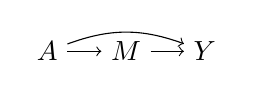
\begin{tikzpicture}
    % x node set with absolute coordinates
    \node (a) at (0,0) {$A$};
    \node (m) at (1,0) {$M$};
    \node (y) at (2,0) {$Y$};
    \path[->] (a) edge (m);
    \path[->] (m) edge (y);
    \path[->, bend left=20] (a) edge (y);
\end{tikzpicture}} seen as longitudinal with  $k_0$: $A$ and $k_1$: $M$


\textbf{decompose} $\mathrm{E}\left[Y^{a=1}\right]  - \mathrm{E}\left[Y^{a=0}\right]$ into cross-world quantities
\begin{itemize}[itemsep=0em, topsep=0pt, partopsep=0pt,parsep=0pt, leftmargin=1.5em]
\item pure (aka natural) direct effect (upper path) $$\mathrm{E}\left[Y^{a=1, M^{a=0}}\right]  - \mathrm{E}\left[Y^{a=0, M^{a=0}}\right]$$
\item total (aka natural) indirect effect (lower path) $$\mathrm{E}\left[Y^{a=1, M^{a=1}}\right]  - \mathrm{E}\left[Y^{a=1, M^{a=0}}\right]$$
\end{itemize}

\textbf{mediation formula} under NPSEM-IE (requires $Y^{a=1,m} \indep M^{a=0}$ cross-world independence)
$$\mathrm{E}\left[Y^{a=1,M^{a=0}}\right] = \sum_m \mathrm{E}\left[Y|A=1, M=m\right]\mathrm{Pr}\left[M=m|A=0\right] $$


\textbf{interventional interpretation} advocating NPSEM-IE assuming:
\trimbox{0cm 0.095cm 0cm 0cm}{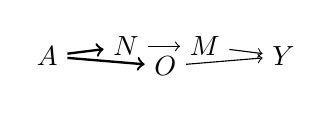
\begin{tikzpicture}
    % x node set with absolute coordinates
    \node (a) at (-1,0.125) {$A$};
    \node (n) at (0,0.25) {$N$};
    \node (o) at (0.5,0) {$O$};
    \node (m) at (1,0.25) {$M$};
    \node (y) at (2,0.125) {$Y$};
    \path[->, line width=0.3mm] (a) edge (n);
    \path[->] (n) edge (m);
    \path[->] (m) edge (y);
    \path[->, line width=0.3mm] (a) edge (o);
    \path[->] (o) edge (y);
\end{tikzpicture}}
(thick arrows are deterministic)

no controlled direct effects: no $N\to Y$ and no $O\to M$

FFRCISTG point of view: intervention on $N$ and $O$ separately

if decomposable (can be verified in a randomized trial), g-formula for $N$ and $O$ reduces to mediation formula for $A$



\end{minipage}}

\end{multicols}


%-------------------------------------------------------------------------------

% SECTION: MODELS

%-------------------------------------------------------------------------------

\section{Models}

\begin{multicols}{2}

\paragraph{Modeling} data are a sample from the target population \vspace{0.4em}

 \hspace{0.9em}\begin{tabular}{l l l}
\textbf{\it estimand:} & quantity  of interest, & e.\,g.\ $\mathrm{E}\left[Y|A=a\right]$ \\
\textbf{\it estimator:} & function to use, & e.\,g.\ $\widehat{\mathrm{E}}\left[Y|A=a\right]$ \\
\textbf{\it estimate:} & apply function to data, & e.\,g.\ $4.1$ 
\end{tabular} \vspace{0.5em}

 \textbf{model}: a priori restriction of joint distribution/dose-response curve;  \textit{assumption:} no model misspecification (usually wrong)

 \textbf{non-parametric estimator:} no restriction (saturated model) $=$ \textit{Fisher consistent estimator} (entire population data $\rightarrow$ true value)

 \textbf{parsimonious model:} few parameters estimate many quantities

 \textbf{bias-variance trade-off:} \newline wiggliness $\uparrow$ $\rightarrow$ misspecification bias $\downarrow$, CI width $\uparrow$

\paragraph{Variable Selection} can induce bias if $L$ includes: 

\hspace{-0.2em}
\begin{tabular}{l l }
 (decendant of) collider:& \textit{selection bias under the null}\\
 noncollider effect of $A$:& \textit{selection bias under the alternative}\\
 mediator:& \textit{overadjustment for mediators}
\end{tabular}

 temporal ordering is not enough to conclude anything

 \textbf{bias amplification:} e.\,g.\ by adjusting for an instrument $Z$ (can also reduce bias)



\paragraph{Super Learning} \citep{van2007super, van2011targeted}

 \textbf{oracle selector:} select best estimator of set of learners $Z_i$

 \textbf{discrete super learner:} select algorithm with smallest cross-validated error (converges to oracle for large sample size)

 \textbf{super learner:} improves asymptotically on discrete version

$\mathrm{logit} (Y=1|Z) = \sum_i \alpha_i Z_i, $ with $0<\alpha_i<1$ and $\sum\alpha_i=1$
weights $\alpha_i$ are determined inside the cross-validation; for the prediction, $Z_i$ trained on the full data set are used

   can be cross-validated itself to check for overfitting (unlikely)


\paragraph{Marginal Structural Models} association is causation in the IP weighted pseudo-population 
$$\text{associational model } \mathrm{E}\left[Y|A\right] = \text{ causal model } \mathrm{E}\left[Y^a\right]$$

 \textit{step 1:} estimate/model $f\left[A|L\right]$ (and $f\left[A\right]$) $\rightarrow$ get $(S)W^A$

 \textit{step 2:} estimate regression parameters for pseudo-population

 \textbf{effect modification} variables $V$ can be included (e.\,g.\ $\beta_0+\beta_1 a+\beta_2 V a + \beta_3 V$; technically not marginal anymore), $SW^A(V) = \frac{f\left[A|V\right]}{f\left[A|L\right]}$ more efficient than $SW^A$
 










\end{multicols}

\subsection{Traditional Methods}

\begin{multicols}{2}




\paragraph{Stratification}  calculate risk for each stratum of $L$

 only feasible if enough data per stratum


\paragraph{Outcome Regression} often assume no effect modification
$$\mathrm{E}\left[Y^{a,c=0}|L\right] = \beta_0 + \beta_1 a + \beta_2 aL +\beta_3 L = \mathrm{E}\left[Y|A, C=0, L\right]$$

 faux marginal structural model as no IP weighting/$SW^A(L)=1$

 for ATE only $\beta_1,\beta_2$ of interest, the rest are \textit{nuisance parameters}

\paragraph{Propensity Score Methods}
$\mathrm{Pr}\left[A=1|L\right] =: \pi(L)$ 
 
  $\Rightarrow A\indep L|\pi(L)$ (definition of a  balancing score); can be modelled  


\begin{itemize}[itemsep=0em, topsep=0pt, partopsep=0pt,parsep=0pt, leftmargin=1.5em]
\setlength{\itemsep}{0pt}%
\setlength{\parskip}{0pt}
\item \textit{\textbf{stratification:}} create strata with similar $\pi(L)$ (e.\,g.\ deciles), but the average $\pi(L)$ might still be different in some strata
\item \textit{\textbf{standardization:}} use $\pi(L)$ instead of $L$ to standardize
\item \textit{\textbf{matching:}} find close ($\rightarrow$ bias-variance trade-off) values of $\pi(L)$, positivity issues arise often
\end{itemize}

 propensity models don't need to predict well, just ensure exchangeability (good prediction leads to positivity problems)


\paragraph{Instrumental Variable Estimation} $L$ unmeasured

 surrogate/proxy instruments can be used

 \textbf{instrumental conditions:} 
\begin{enumerate}[itemsep=0em, topsep=0pt, partopsep=0pt,parsep=0pt, leftmargin=1.5em]
\setlength{\itemsep}{0pt}%
\setlength{\parskip}{0pt}
\item \textbf{\textit{relevance condition:}} $Z \not\!\indep A$, meaning $Z$ is associated with $A$ \newline (weak association (F-statistic $< 10$) $\rightarrow$ weak instrument)
\item \textbf{\textit{exclusion restriction:}} $Z$ affects $Y$ at most through $A$
\begin{enumerate}[itemsep=0em, topsep=0pt, partopsep=0pt,parsep=0pt, leftmargin=1.5em]
\setlength{\itemsep}{0pt}%
\setlength{\parskip}{0pt}
\item population level: $\mathrm{E}\left[Y^{z,a}\right] = \mathrm{E}\left[Y^{z',a}\right]$ (sometimes enough)
\item \textbf{\textit{individual level:}} $Y^{z,a}_i =  Y^{z',a}_i = Y^{a}_i$
\end{enumerate}
\item \textbf{\textit{exchangeability:}} $Z$ and $Y$ have no shared causes
\begin{enumerate}[itemsep=0em, topsep=0pt, partopsep=0pt,parsep=0pt, leftmargin=1.5em]
\setlength{\itemsep}{0pt}%
\setlength{\parskip}{0pt}
\item \textbf{\textit{marginal:}} $Y^{a,z} \indep Z$ (typically enough)
\item joint: $\left\{Y^{z, a};a\in\left[0,1\right],z\in\left[0,1\right]\right\} \indep Z$
\end{enumerate}
\item  (not needed for an instrument, just the IV estimand below)
\begin{enumerate}[itemsep=0em, topsep=0pt, partopsep=0pt,parsep=0pt, leftmargin=1.5em]
\setlength{\itemsep}{0pt}%
\setlength{\parskip}{0pt}
\item \textit{effect homogeneity:} (i) constant effect $A\rightarrow Y \,\, \forall i$ (ii) constant average effect $A\rightarrow Y \,\, \forall A$ (iii) no additive effect modifiers (iv) additive Z-A association is constant across $L$
\item \textit{monotonicity:} $A^{z=1} \geq A^{z=0} \,\, \forall i$ (more credible than 4a)
\end{enumerate}
\end{enumerate}

 \textbf{common instruments:} (physician's) general preference, access to/price of $A$, genetic factors (Mendelian randomization)

 \textbf{bounds:} binary outcome ATE $\left[-1,1\right]$ (width 2)  $\overset{data}{\rightarrow}$ (width 1)

 \textit{natural bounds} need 2a,3a  (width $\mathrm{Pr}\left[A{=}1|Z{=}0\right] + \mathrm{Pr}\left[A{=}0|Z{=}1\right]$)

 \textit{sharp bounds} require 2a,3b (narrower than natural bounds)


 \textbf{IV estimand ATE}: intention-to-treat $\div$ measure of compliance

 (1,2b,3a,4a):  ATE;
  (1,2b,3a,4b): ATE in compliers

 binary $Z$: $\frac{\mathrm{E}\left[Y|Z=1\right] - \mathrm{E}\left[Y|Z=0\right]}{\mathrm{E}\left[A|Z=1\right] - \mathrm{E}\left[A|Z=0\right]}$, continuous $Z$: $\frac{Cov(Y,Z)}{Cov(A,Z)}$; \newline can be calculated as \textit{two-stage-least-squares estimator:} \newline 1.\ $\mathrm{E}\left[A|Z\right]$ 2.\ $\mathrm{E}\left[Y|Z\right] = \beta_0 + \beta_1\hat{\mathrm{E}}\left[A|Z\right]$ 3. $\hat{\beta}_1$ is IV estimate

 \textbf{disadvantages:} often leads to wide CI, small violations of conditions can lead to large biases

 \textbf{regression discontinuity design:} if threshold in $L$ exists which determines $A$ perfectly + assumption of continuity in $L$ $\to$ jump in $Y$ at threshold is the causal effect (if no effect modification by $L$); a fuzzy variant also exists
\citep{hernan2023causal}



\paragraph{Causal Survival Analysis} time-to-event data

 additional censoring due to administrative end of follow-up

 \textbf{competing events} (often death): censoring (assume population with death abolished) or not (after death, chance of event is zero, but what is the effect of $A$?) $\rightarrow$ create composite event

 \textbf{survival quantities} $k$ is a time point, $T$ is time of event
\begin{itemize}[itemsep=0em, topsep=0pt, partopsep=0pt,parsep=0pt, leftmargin=1.5em]
\setlength{\itemsep}{0pt}%
\setlength{\parskip}{0pt}
\item \textit{survival} at $k$: $\mathrm{Pr}\left[T>k\right] =:\mathrm{Pr}\left[D_k=0\right]$
\item \textit{risk} at $k$: $1-\mathrm{Pr}\left[T>k\right] = \mathrm{Pr}\left[T \leq k\right] = \mathrm{Pr}\left[D_k=1\right]$
\item \textit{hazard} at $k$: $\mathrm{Pr}\left[T=k|T> k{-}1\right] =\mathrm{Pr}\left[D_k=1|D_{k{-}1}=0\right]$, \textit{hazard ratio} is paradoxical due to  in-built selection bias
\end{itemize}

 \textbf{modeling:} some options
\begin{itemize}[itemsep=0em, topsep=0pt, partopsep=0pt,parsep=0pt, leftmargin=1.5em]
\setlength{\itemsep}{0pt}%
\setlength{\parskip}{0pt}
\item \textit{\textbf{Kaplan-Meier}} aka product limit formula (nonparametric): $\mathrm{Pr}\left[D_k=0\right] = \prod_{m=1}^k \mathrm{Pr}\left[D_m=0|D_{m-1}=0\right]$
\item parametric e.\,g.\ log hazards model: 
\begin{itemize}[itemsep=0em, topsep=0pt, partopsep=0pt,parsep=0pt, leftmargin=1.5em]
\setlength{\itemsep}{0pt}%
\setlength{\parskip}{0pt}
\item use \textit{\textbf{IP weigths}} $SW^A$ in structural marginal model $\mathrm{logit} \: \mathrm{Pr}\left[D_{k+1}^{a, \bar{c}=\bar{0}}=0|D_{k}^{a, \bar{c}=\bar{0}}=0\right] = \beta_{0,k} + \beta_1a+\beta_2ak $
\item \textit{\textbf{standardize}} ($\prod_k 1-$) parametric hazards model $\mathrm{Pr}\left[D_{k+1}=1|D_k = 0, C_k=0, L, A\right]$ weighting across $L$
\end{itemize}
\item \textit{\textbf{structural nested cumulative failure time model (CFT):}}
$\frac{\mathrm{Pr}\left[D_k^a=1|L,A\right]}{\mathrm{Pr}\left[D_k^{a=0}=1|L,A\right]} = \exp\left[\gamma_k(L,A;\psi)\right]$ (log-linear has no upper limit 1 $\rightarrow$ rare failure $\uparrow$; if $\downarrow$, use a survival model (CST)), use g-estimation like with AFT
\item \textit{\textbf{accelerated failure time model (AFT)}} with g-estimation: $T_i^a/T_i^{a=0} = \exp(-\psi_1a -\psi_2aL_i)$, exchangeability for $C$ is guaranteed via artificial censoring (include only individuals who would not have been censored either way) 
\end{itemize}



\vspace{0.2em}
 \colorbox{lightgray!20!white}{\begin{minipage}{28em}




\textbf{\textcolor{darkgray}{time-varying}} two options based on g-methods as examples

 \textbf{standardization} (plug-in estimate): risk is $\mathrm{Pr}\left[D_{k+1}^{\bar{a},\bar{c}=\bar{0}}=1\right] =$ \vspace{-0.5em}
\begin{align*}%{3}
 \sum_{\bar{l}_k}&\sum_{j=0}^k \mathrm{Pr}\left[D_{j+1}=0|\bar{A}_j=\bar{a}_j, \bar{L}_j=\bar{l}_j, \bar{D}_j=0\right] \times \\[-0.1em]
\prod_{s=0}^j & \Big\{  \mathrm{Pr}\left[D_s=0|\bar{A}_{s-1}=\bar{a}_{s-1}, \bar{L}_{s-1}=\bar{l}_{s-1}, \bar{D}_{s-1}=0\right] \times  \\[-0.7em]
   &   \,\,\,\,\, f\left(l_s|\bar{a}_{s-1}, \bar{l}_{s-1}, D_s=0\right)\Big\}
\end{align*}
 \textbf{IP weighting:} fit a pooled logistic hazard model with time-varying weights
$W^{\bar{A}}_k =\prod_{m=0}^k\frac{1}{f(A_m|\bar{A}_{m-1}, \bar{L}_m)}$



\end{minipage}}



\end{multicols}


%-------------------------------------------------------------------------------

% SECTION: G-METHODS

%-------------------------------------------------------------------------------

\subsection{G-Methods}
\begin{multicols}{2}


\paragraph{G-Methods} \textit{g}eneralized treatment contrasts:
adjust for $L$
\begin{itemize}[itemsep=0em, topsep=0pt, partopsep=0pt,parsep=0pt]
\setlength{\itemsep}{0pt}%
\setlength{\parskip}{0pt}
\item \textbf{\textit{standardization:}}  two types of g-formula
\item \textbf{\textit{IP weighting:}} (in theory) also g-formula 
\item \textbf{\textit{g-estimation:}} not needed unless longitudinal
\end{itemize}

 \textbf{standardization and IP weighting}
are equivalent, \textit{\textbf{but}} if modeled, different ``no misspecification'' assumptions: outcome model (standardization), treatment model (IP weighting)

 \textbf{big g-formula}
not all methods use (sequential) exchangeability 
\begin{itemize}[itemsep=0em, topsep=0pt, partopsep=0pt,parsep=0pt]
\item \textit{problem:} DAG is known, but unmeasured variables exist
\item \textit{solution:} include un- \& measured variables in big g-formula $\to$ derive
alternative effect identification methods using only d-separation (e.\,g.\  front door formula)
\end{itemize}
it can always be determined, if the DAG allows for identification with the big g-formula
\citep{hernan2023causal}


 \textbf{censoring:} measure joint effect of $A$ and $C$ with
$\mathrm{E}\left[Y^{a, c=0}\right]$

 \textit{standardization} $\mathrm{E}\left[Y|A=a\right] = \int \mathrm{E}\left[Y|L{=}l, A{=}a, C{=}0\right]dF_L\left[l\right]$\vspace{0.2em}

 \textit{IP weights}\vspace{-1.30em}

\hspace{4.3em}\begin{tabular}{l l l}
$W^{A,C}=W^A \times W^C$  &(uses $n$) & or \\
$SW^{A,C}=SW^A \times SW^C$ &(uses $n^{c=0}$) & 
\end{tabular}\vspace{0.3em}

 \textit{g-estimation} only adjusts for confounding  $\rightarrow$ use IP weights

\vspace{0.2em}
 \colorbox{lightgray!20!white}{\begin{minipage}{28em}

\textbf{\textcolor{darkgray}{time-varying}} censoring $\bar{C}$: monotonic type of missing data 

 \textbf{standardization}: $\!\!\!\displaystyle\int\!\! f(y|\bar{a}, \bar{c}{=}\bar{0}, \bar{l}) \prod\limits_{k=0}^K dF\left(l_k|\bar{a}_{k-1}, c_{k-1} {=} 0, \bar{l}_{k-1}\right)$

 \textbf{IP weighting}:
 $$\textcolor{gray}{S}W^{\bar{C}}= \prod_{k=1}^{K+1}\frac{1\textcolor{gray}{\cdot \mathrm{Pr}\left(C_k=0|\bar{A}_{k-1}, C_{k-1}=0\right)}}{\mathrm{Pr}\left(C_k=0|\bar{A}_{k-1}, C_{k-1}=0, \bar{L}_k\right)} $$

\end{minipage}}




\paragraph{Standardization} plug-in (parametric if so) g-formula
$$\mathrm{E}\left[Y^{a}\right] = \overbrace{\mathrm{E}\left[\mathrm{E}\left[Y|A{=}a,L{=}l\right]\right]}^{\text{conditional expectation}} =  \overbrace{ \textstyle{\int} \mathrm{E}\left[Y|A=a, L=l\right]f_L\left[l\right]dl}^{\text{joint density estimator}} $$
weighted average of stratum-specific risks; unknowns can be estimated non-parametrically or modeled

 \textbf{no need to estimate $\boldsymbol{f_L\left[l\right]}$/integrate} as empirical distribution can be used: estimate outcome model $\rightarrow$ predict counterfactuals on whole dataset $\rightarrow$ average the results ($\rightarrow$ CI by bootstrapping)

 \textbf{for discrete $\boldsymbol{ L}$}  $\mathrm{E}\left[Y|A=a\right]$ is $\sum_l \mathrm{E}\left[Y|A=a,L=l\right]\mathrm{Pr}\left[L=l\right]$

\vspace{0.2em}
 \colorbox{lightgray!20!white}{\begin{minipage}{28em}

\textbf{\textcolor{darkgray}{time-varying}} standardize over all possible $\bar{l}$-histories



 simulates joint distribution of counterfactuals $\left(Y^{\bar{a}}, \bar{L}^{\bar{a}}\right)$ for $\bar{a}$
\textbf{joint density estimator (jde)}
\begin{align*}
& \text{discrete: } \mathrm{E}\left[Y^{\bar{a}}\right] = \sum_{\bar{l}} \mathrm{E}\left[Y|\bar{A}=\bar{a}, \bar{L}=\bar{l} \right] \prod_{k=0}^K f \left(l_k|\bar{a}_{k-1}, \bar{l}_{k-1}\right)  \\ &
\text{continuous: } \int f(y|\bar{a}, \bar{l}) \prod_{k=0}^K f\left(l_k|\bar{a}_{k-1}, \bar{l}_{k-1}\right)dl
\end{align*}

 for \textit{stochastic strategies} multiply with $\prod_{k=0}^K f^{int} \left(a_k|\bar{a}_{k-1}, \bar{l}_{k}\right) $

\end{minipage}}

 \colorbox{lightgray!20!white}{
\begin{minipage}{28em}


\begin{mdframed}[linecolor=black!20!,
    outerlinewidth=0.2pt,
    innertopmargin=0.5\baselineskip,
    innerbottommargin=0.5\baselineskip,
    backgroundcolor=lightgray!20!white, innerleftmargin=2pt, innerrightmargin=2pt]
\textbf{estimation} \citep{young2011comparative, schomaker_using_2019}

\begin{enumerate}[itemsep=0em, topsep=0pt, partopsep=0pt,parsep=0pt, leftmargin=1.5em]
\setlength{\itemsep}{0pt}%
\setlength{\parskip}{0pt}
\item model $f \left(l_k|\bar{a}_{k-1}, \bar{l}_{k-1}\right)$ and $\mathrm{E}\left[Y|\bar{A}=\bar{a}, \bar{L}=\bar{l} \right]$
\item simulate data forward in time: \newline
at $k=0$: use empirical distribution of $L_0$ (observed data) \newline
at $k>0$: set $\bar{A} = \bar{a}$, \textit{draw} from models estimated in 1.
\item calculate mean of $\hat{Y}_{K,i}^{\bar{a}}$ (bootstrap for CI)
\end{enumerate}

\end{mdframed}





\textbf{iterated conditional expectation (ice)} 
$$\mathrm{E}\left[ Y_T^{\bar{a}}\right] = \mathrm{E} \left[ \mathrm{E} \left[\mathrm{E} \left[ ... \mathrm{E} \left[Y_T| \bar{A}_{T{-}1} {=} \bar{a}_{T{-}1}, \bar{L}_T \right]  ...|\bar{A}_0 {=} a_0, L_1 \right] |L_0 \right]\right]$$



\begin{mdframed}[linecolor=black!20!,
    outerlinewidth=0.2pt,
    innertopmargin=0.5\baselineskip,
    innerbottommargin=0.5\baselineskip,
    backgroundcolor=lightgray!20!white, innerleftmargin=2pt, innerrightmargin=2pt]
\textbf{estimation} \citep{schomaker_using_2019}

\begin{enumerate}[itemsep=0em, topsep=0pt, partopsep=0pt,parsep=0pt, leftmargin=1.5em]
\setlength{\itemsep}{0pt}%
\setlength{\parskip}{0pt}
\item model inside out: $Q_{T} {=} \mathrm{E} \left[Y_T| \bar{A}_{T{-}1}, \bar{L}_T \right]$ to $Q_0 {=} \mathrm{E} \left[Q_1| \bar{L}_0 \right]$, predict $Q_t$ with $\bar{A} = \bar{a}$ in each step
\item calculate mean of $\hat{Q}_{0,i}^{\bar{a}}$ (bootstrap for CI)
\end{enumerate}



\end{mdframed}

 \textbf{g-null paradox} even if the sharp null holds, model misspecification can lead to it being falsely rejected

\end{minipage}}



\begin{mdframed}[style=MyFrame,nobreak=true, innerleftmargin=2pt, innerrightmargin=2pt]
Proof: for $L_0 \rightarrow A_0 \rightarrow Y_0 \rightarrow L_1 \rightarrow A_1 \rightarrow Y_1$, $\bar{a} =(a_0,a_1)$ 
\begin{alignat*}{4} 
\mathrm{E}\left[Y_1^{\bar{a}}\right] & \overset{\text{CE}}{=} && \mathrm{E}\left[\mathrm{E}\left[   Y_1^{\bar{a}}|A_0{=}a_0, L_0   \right]\right]  \\ 
\text{(ice)}\,\,\, &\overset{\text{CE*}}{=} && \mathrm{E}\left[\mathrm{E}\left[  \mathrm{E}\left[Y_1|\bar{L}, \bar{A}{=}\bar{a}, Y_0 \right]| A_0{=}a_0, L_0   \right]\right]  \\ 
&\overset{\text{LIE}}{=} && \mathrm{E}\left[ \sum\nolimits_{l_1} \mathrm{E}\left[Y_1|A_0{=}a_0, \bar{L}, Y_0\right] \mathrm{Pr}\left[l_1|a_0,l_0, y_0\right]         \right] \\
&\overset{\text{LIE}}{=} && \sum\nolimits_{l_0}\!\!\!\left[ \sum\nolimits_{l_1} \!\!\!\mathrm{E}\left[Y_1|A_0{=}a_0, \bar{L}, Y_0\right] \mathrm{Pr}\left[l_1|a_0,l_0, y_0\right]         \right] \mathrm{Pr}\left[l_0\right] \\
\text{(jde)}\,\,\, &\overset{\text{sum}}{=} &&  \sum\nolimits_{\bar{l}} \mathrm{E}\left[Y_1|A_0{=}a_0, \bar{L}, Y_0\right] \mathrm{Pr}\left[l_1|a_0,l_0\right]          \mathrm{Pr}\left[l_0\right] 
\end{alignat*}
CE: conditional expectation; *: exchangeability; \newline LIE: law of iterated expectation
\end{mdframed}







\paragraph{IP Weighting} \textit{i}nverse \textit{p}robability of treatment (g-formula)
$$\mathrm{E}\left[Y^{a}\right] = \mathrm{E}\left[\frac{I(A=a)Y}{f\left[A|L\right]}\right]; W^A=\frac{1}{f\left[A|L\right]}; SW^A = \frac{f(A)}{f\left[A|L\right]}$$

 unknowns can be estimated non-parametrically or modeled
 \textbf{pseudo-population:} everyone is treated \& untreated ($L\not\to A$)

 \textbf{FRCISTG} \textit{(fully randomized causally interpreted structured graph)}: probability tree for $L \rightarrow A \rightarrow Y$, can be used to calculate/visualize simulation of values for $A$ 

 \textbf{for discrete $\boldsymbol{A, L}$:} $f\left[a|l\right] = \mathrm{Pr}\left[A=a,L=l\right]$

 \textbf{estimators:} Horvitz-Thompson; Hajek (modified version) %todo p.152 

 \textbf{stabilized weights $\boldsymbol{SW^A}$} should have an average of 1 (check!) $\rightarrow$ pseudo-population same size $\rightarrow$ (if non-saturated) CI width $\downarrow$ 

\vspace{0.2em}
 \colorbox{lightgray!20!white}{\begin{minipage}{28em}




\textbf{\textcolor{darkgray}{time-varying}}
$$ W^{\bar{A}} = \prod_{k=0}^K \frac{1}{f\left(A_k|\bar{A}_{k-1}, \bar{L}_k\right)}; \,\,\,\, SW^{\bar{A}} = \prod_{k=0}^K \frac{f\left(A_k|\bar{A}_{k-1}\right)}{f\left(A_k|\bar{A}_{k-1}, \bar{L}_k\right)}$$

\end{minipage}}



















\paragraph{G-Estimation} (additive) structural nested models %todo: verbesserung von allem, ich habs noch nicht ganz verstanden
\begin{align*}
\mathrm{logit} \, \mathrm{Pr}\left[A=1|H(\psi^\dagger), L\right] &= \alpha_0 + \alpha_1H(\psi^\dagger) + \alpha_2L \\
H(\psi^\dagger) &= Y - \psi_\dagger A
\end{align*}
find $\psi^\dagger$ which renders $\alpha_1=0$; 95\,\%-CI: all $\psi^\dagger$ for which $p>0.05$
closed-form solution for linear models


 \textbf{derivation:} $H(\psi^\dagger) = Y^{a=0}$
$$\mathrm{logit} \, \mathrm{Pr}\left[A=1|Y^{a=0}, L\right] = \alpha_0 + \alpha_1Y^{a=0} + \alpha_2L$$
$Y^{a=0}$ unknown, but because of exchangeability $\alpha_1$ should be zero
$$Y^{a=0} =Y^a - \psi_1 a$$
equivalent to $Y^{a=0} =Y^{a=1} - \psi_1$, but using no counterfactuals



 \textbf{structural nested mean model}
\begin{align*}
\text{additive: }\,\,\, & \mathrm{E}\left[Y^a-Y^{a=0}|A=a, L\right] &= \beta_1 a \,(+ \beta_2 a L) \\
\text{multiplicative: }\,\,\, & \log \left( \frac{\mathrm{E}\left[Y^a|A=a, L\right]}{\mathrm{E}\left[Y^{a=0}|A=a, L\right]} \right) &= \beta_1 a \,(+ \beta_2 a L)
\end{align*} 
multiplicative is preferred if $Y$ always positive, but does not extend to longitudinal case

 semi-parametric: agnostic about $\beta_0$ and effect of $L$ $\rightarrow$ robust $\uparrow$

 \textbf{no time-varying:} no nesting; model equals marginal structural models with missing $\beta_0, \beta_3$ (unspecified ``no treatment'')

 \textbf{sensitivity analysis:} unmeasured confounding ($\alpha_1 \neq 0$) can be examined: do procedure  for different values of $\alpha_1$ $\rightarrow$ plot $\alpha_1$ vs.\ $\psi^\dagger$ $\rightarrow$ how sensitive is  estimate to unmeasured confounding?

 \textbf{effect modification:} add $V$ in both g-estimation equations %todo


 \textbf{doubly robust estimators} exist%todo

\vspace{0.2em}
 \colorbox{lightgray!20!white}{\begin{minipage}{28em}
\textbf{\textcolor{darkgray}{time-varying}}
 nested equations: for each time $k$

 \textbf{strutural nested mean models} separate effect of each $a_k$
$$\mathrm{E}\left[Y^{\bar{a}_{k-1}, a_k, \underline{0}_{k+1}} - Y^{\bar{a}_{k-1}, \underline{0}_{k+1}}|\bar{L}^{\bar{a}_{k-1}}=\bar{l}_k, \bar{A}_{k-1} = \bar{a}_{k-1}\right] = $$
$$  a_k\gamma_k\left(\bar{a}_{k-1}, \bar{l}_k,\beta\right)$$
 \textbf{calculations}
$$H_k\left(\psi^\dagger\right) = Y - \sum_{j=k}^K A_j \gamma_j\left(\bar{A}_{j-1}, \bar{L}_j, \psi^\dagger\right)$$
 function $\gamma_j$ can be, e.\,g.\ constant ($\psi_1$), time-varying only ($\psi_1+\psi_2k$), or dependent on treatment/covariate history
$$\mathrm{logit}\,\mathrm{Pr}\left[A_k=1|H_k\left(\psi^\dagger\right), \bar{L}_k,\bar{A}_{k-1}\right]=$$
$$\alpha_0 +\alpha_1H_k\left(\psi^\dagger\right)+\alpha_2 w_k\left(\bar{L}_k,\bar{A}_{k-1}\right)
$$
find $\alpha_1$ that is closest to zero

a closed form estimator exists for the linear case

\end{minipage}}

























\end{multicols}



\subsection{Doubly Robust Methods}

\begin{multicols}{2}



\paragraph{Double-Robustness} \citep{hernan2023causal}

 g-formula: \textit{either} treatment model $f(L)$  \textit{or} outcome model $b(L)$ 

 \textit{\textbf{or}} appropriately combine both: ``two chances to get it right''

 \textbf{all doubly robust estimators} 
\begin{itemize}[leftmargin=*, itemsep=0em, topsep=0pt, partopsep=0pt,parsep=0pt]
\item involve a correction of  outcome $\hat{b}(L)$ using the treatment $\hat{f}(L)$
\item have a bias depending on a product of the errors $\frac{1}{\pi(l)} - \frac{1}{\hat{\pi}(l)}$ and $b(l) - \hat{b}(l)$ known as second order bias 
%(as discussed in chapter 18, this allows machine learning, as machine learning will get that bias smaller than other things in high-dimensional cases)
\end{itemize}

\vspace{0.2em}
 \colorbox{lightgray!20!white}{\begin{minipage}{28em}

\textbf{\textcolor{darkgray}{time-varying:}} 
  multiple robustness for $k=0,1,...K$
  
 $K{+}\,2$ robustness: consistent, if $\hat{f}_0$ to $\hat{f}_l$ and $\hat{b}_{l+1}$ to $\hat{b}_K$ are 
 
 $2^{K{+}1}$ robustness: consistent, if for each k, either  $\hat{f}_k$ or $\hat{b}_k$ are
  
  \end{minipage}}

\paragraph{Machine Learning} $L$ is high-dimensional

 one could use lasso or ML for IP weighting/standardization

 \textbf{\textit{but:}} ML does not guarantee elimination of confounding and has largely unknown statistical properties: how to get CI?

 \textbf{sample splitting:} train estimators on training sample $T_r$, use resulting estimators for doubly robust method on estimation sample (CIs on estimation sample are valid, but $n$ halved)

 \textbf{cross-fitting:} do again the other way round, average the two estimates, get CI via bootstrapping
[\textit{alternatively:} split into $M$ samples, use one sample for estimation and $M{-}1$ for training $\to$ improved finite sample behavior \citep{hernan2023causal}]



 \textbf{asymptotic behavior} 
for valid (Wald) CI we need:
\begin{itemize}[leftmargin=*, itemsep=0em, topsep=0pt, partopsep=0pt,parsep=0pt]
\item a bias  much smaller than $c \cdot 1/\sqrt{n}$, which is how the $se$ typically scales (use doubly robust methods for small bias)
%Wald CI for $\mathrm{E}\left[Y^a\right] $ standard error typically scales as $c \cdot 1/\sqrt{n}$, therefore, the bias needs to be much less for valid CI 
\item asymptotic normality (for Wald CI)
\item for a doubly robust estimator $\psi_{dr}$, we need sample splitting, otherwise $\hat{b}(l)$ and $\hat{f}(l)$ are correlated with $\psi_{dr}$
\end{itemize}

 if $\hat{b}(l)$ and $\hat{f}(l)$ are consistent and $\mathrm{E}[\hat{\psi} - \psi|T_r]/se(\hat{\psi})$ converges to 0 $\to$ $\hat{\psi}$ with sample splitting is asymptotically normal and unbiased $\to$ CI is calibrated
\citep{hernan2023causal}


 \textbf{problems:} unclear choice of algorithm, is bias small enough?

\paragraph{Advantages} \citep{van2011targeted}

 \textbf{consistent} \textit{if either $\bar{Q}_0$ or $g_n$ are consistent (doubly robust)}:
$$\forall \epsilon>0, P \in \mathcal{M}: \mathrm{Pr}_P\left[|\hat{\theta}_n-\theta(P)|>\epsilon\right] \to 0 \text{ as } n\to\infty$$

 \textbf{collaboratively doubly robust:} $g_n$ only needs predictors of $Y$, as it does not try to fit $g_0$ well, but improve the fit of $\bar{Q}^*_n$

 \textbf{asymptotic unbiasedness}
\textit{if either $\bar{Q}_0$ or $g_0$ are consistent}, super learning makes $\bar{Q}_0$ and $g_n$ max.\ asymptotically unbiased

 \textbf{asymptotic efficiency} \textit{if both $\bar{Q}_0$ and $g_n$ are consistent}: achieves Cramer-Rao bound of minimum possible asymptotic variance (requires asymptotic unbiasedness)

 \textbf{asymptotic linearity} \textit{if either  $\bar{Q}_0$ or $g_n$ are consistent}: \newline means estimator behaves like empirical mean
\begin{itemize}[leftmargin=*, itemsep=0em, topsep=0pt, partopsep=0pt,parsep=0pt]
\setlength{\itemsep}{0pt}%
\setlength{\parskip}{0pt}
\item bias converges to zero at rate smaller than $1/\sqrt{n}$
\item for large $n$ estimator is approximately normally distributed
\end{itemize}

\paragraph{Influence Curve} how robust is an estimator? %\citep{hampel1974influence, van2011targeted}
$$IC_{T,P_n}(O)=\lim_{\epsilon\to 0}\frac{T\left[\left(1-\epsilon\right)P_n + \epsilon\delta_O\right]-T(P_n)}{\epsilon}$$
for estimator $T$ and distribution $P_n$ with $0<\epsilon<1$ 


 can also be rewritten as a \textit{\textbf{directional derivative}} at $P_n$
$$IC_{T,P_n}=\frac{d}{d\epsilon}T\left[\left(1-\epsilon\right)P_n + \epsilon\delta_O\right] = 
\frac{d}{dP_n}T\left(\delta_O - P_n\right)$$
in direction $(\delta_O - P_n)$, where $P_n$ empirical probability measure that puts mass $1/n$ on $O_i$ \citep{hampel1974influence}


 \textbf{special cases} \citep{van2011targeted}
\begin{itemize}[leftmargin=*, itemsep=0em, topsep=0pt, partopsep=0pt,parsep=0pt]
\item $\overline{IC}(P_0) = 0$ and $\mathrm{Var}(IC(P_0))$ asymptotic variance of the standard estimator  $\sqrt{n} (\psi_n - \psi_0)$, $\to$ $Var(\hat{\Psi}(P_n)) = \frac{Var_{IC}}{n}$
\item efficient IC: an estimator is asymptotically efficient $\Leftrightarrow$ its influence curve is the efficient influence curve $IC(O)=D^*(O)$ 
\end{itemize}





\paragraph{Delta Method}  \citep{zepeda2022delta} estimand is a function of $\theta$, i.e. $\psi := \phi(\theta)$, $Var(\hat{\theta})$ known, but what is $Var(\hat{\psi})$?


 \textbf{Taylor's approximation} requirements:
\begin{itemize}[leftmargin=*, itemsep=0em, topsep=0pt, partopsep=0pt,parsep=0pt]
\item univariate $\phi$: differentiable at $\theta$
\item multivariate $\phi$: $\exists$ $\partial_v\phi(\theta)$ (directional derivative)
\item functional $\phi$ (function of functions): $\exists$ $\partial_v\phi(\theta)$ \& coincides with one-sided directional (Hadamard) derivatives ($\overset{*}{=}\nabla \phi(\theta)^Tv$)
\end{itemize}

 first order Taylor \textcolor{gray}{(rearranged$^\dagger$)}: $\phi(\hat{\theta}_n) \overset{\mathbin{\textcolor{gray}{-}}}{\approx} \phi(\theta) \overset{\mathbin{\textcolor{gray}{\approx}}}{+} \partial_{v:=\hat{\theta}-\theta}\phi(\theta)$

 \textbf{classical delta method:} if $\{r_n\}_{n=1}^\infty$ with $\lim_{n\to\infty} r_n=\infty$, where $r_n(\hat{\theta}_n -\theta)$ converges to $Z {\sim} \mathrm{N}(0,1)$ (e.\,g.\  $r_n{=}\sqrt{n/\sigma^2}$), then
$$r_n\left(\phi(\hat{\theta}_n) -\phi(\theta)\right) \overset{\mathbin{\textcolor{gray}{\dagger}}*}{\approx} \nabla \phi(\theta)^Tr_n(\hat{\theta}_n - \theta)    \overset{d}{\to} \nabla \phi(\theta)^TZ$$
$\Rightarrow$ $\mathrm{Var}\left[\phi(\hat{\theta}_n) {-}\phi(\theta)\right] = \mathrm{Var}\left[\phi(\hat{\theta}_n)\right]\approx \frac{1}{r^2_n} \mathrm{Var}\left[\nabla\phi(\theta)^TZ\right]$

 \textbf{functional delta:} $r_n(\hat{\theta}_n {-} \theta) \overset{d}{\to}Z$ $\Rightarrow$ 
$r_n\!\left(\phi(\hat{\theta}_n) {-} \phi(\theta)\right) \overset{d}{\to}\partial_Z\phi(\theta)$

 \textbf{influence function:} $\psi = \phi(\mathbb{P}_X)$ is a functional

% $\hat{\psi} = \phi(\hat{\theta}) = \phi(\hat{\mathbb{P}}_X) $ with $\hat{\mathbb{P}}_X$ empirical PMF (plug-in estimator)

 estimations rate of change for $\mathbb{P}_X$ to $Q$, where $Q=\mathbbm{1}_{\{Y\}}$
$$\mathrm{IF}_{\phi, \mathbb{P}_X}(Y) := \partial_{Q-\mathbb{P}_X}\phi(\mathbb{P}_X) =\lim_{h\downarrow 0}\frac{\phi\left((1-h)\mathbb{P}_X + hQ\right)-\phi(\mathbb{P}_X)}{h},$$



 \textit{interpretation:} rate of change if distribution deviates from $\mathbb{P}_X$ to $Q=$  one observation $Y$, assigns probability 1 to $X$ taking  value $Y$ 

 \textit{use delta:} $\phi(\hat{\mathbb{P}}_X) \approx \phi(\mathbb{P}_X) + \mathrm{IF}_{\phi, \mathbb{P}_X}(Y)$, if $(\hat{\theta}_n - \theta) \overset{n\to\infty}{\sim} \mathrm{N}(.,.)$
$$\hat{\psi}_n - \psi = \phi(\hat{\theta}_n)-\phi(\theta) \overset{\text{approx}}{\sim} \mathrm{N}\left(0, \mathrm{Var}[\mathrm{IF}_{\phi, \mathbb{P}_X}(Y)]\right),$$
where
$\widehat{\mathrm{Var}}[\mathrm{IF}_{\phi, \mathbb{P}_X}(Y)] = \frac{1}{n}\sum_{i=1}^n \left(\mathrm{IF}_{\phi, \mathbb{P}_X}(X_i)\right)^2$, which is the classical $S^2$ estimator since the mean is known ($=0$)

 \textbf{using the delta method (general case)}
\begin{enumerate}[leftmargin=*, itemsep=0em, topsep=0pt, partopsep=0pt,parsep=0pt]
\item determine asymptotic distribution of $v:=r_n(\hat{\theta}_n -\theta)$
\item define $\phi$ and compute Hadamard derivative
\item multiply asymptotic distribution with Hadamard derivative, then estimate the variance
\end{enumerate}


\paragraph{Simple Plug-In Estimator} proto-TMLE   \vspace{-0.3em}

1. fit outcome regression with variable $R = \begin{cases} +W^A & \text{if } A{=}1 \\ -W^A & \text{if } A{=}0 \end{cases}$ \vspace{-0.9em}

2. standardize by averaging


\vspace{0.2em}
 \colorbox{lightgray!20!white}{\begin{minipage}{28em}

\textbf{\textcolor{darkgray}{time-varying}}  $K+2$ robust estimator (related to TMLE)
\begin{enumerate}[leftmargin=*, itemsep=0em, topsep=0pt, partopsep=0pt,parsep=0pt]
\setlength{\itemsep}{0pt}%
\setlength{\parskip}{0pt}
\item 
estimate $\hat{f}\left(A_m|\bar{A}_{m-1}, \bar{L}_m\right)$ (e.\,g.\ logistic model), use it to \newline
calculate at each time $m$: $\widehat{W}^{\bar{A}_m} = \prod_{k=0}^m\frac{1}{\hat{f}\left(A_k|\bar{A}_{k-1}, \bar{L}_k\right)}$ and modified IP weights at $m$: $\widehat{W}^{\bar{A}_{m-1, a_m}} = \frac{\widehat{W}^{\bar{A}_{m-1}}}{\hat{f}\left(a_m|\bar{A}_{m-1}, \bar{L}_m\right)} $
\item with $\widehat{T}_{K+1}:=Y$, recursively for $m=K, K-1, ..., 0$:\newline
 (a) fit outcome regression on $\widehat{T}_{m+1}$ with variable  $\widehat{W}^{\bar{A}_m}$\newline
 (b) calculate $\widehat{T}_{m}$ using the outcome model with $\widehat{W}^{\bar{A}_{m-1, a_m}}$
\item calculate standardized mean outcome $\widehat{\mathrm{E}}\left[Y^{\bar{a}}\right] = \mathrm{E}\left[\widehat{T}_0\right]$
\end{enumerate}

\end{minipage}}


\paragraph{Augmented IPTW} \citep{hernan2023causal}
\begin{align*}
\hat{\mathrm{E}}\left[Y^{a}\right] &= \frac{1}{n}\sum_{i=1}^n\left[
\frac{\mathbbm{1}(A=a)Y}{\hat{f}(A|L)} - \left(\frac{\mathbbm{1}(A=a)}{\hat{f}(A|L)} -1\right)\hat{b}(a,L)
\right]  %\\
%&= P_n \left[ \hat{b}(a,L) + \frac{\mathbbm{1}(A=a)\left\{Y-\hat{b}(A,L)\right\}}{\hat{f}(A|L)}\right]
\end{align*}

 
 \textbf{disadvantages}: ignores global constraints $\to$ often unstable if sparsity, sometimes not well-defined \citep{van2011targeted}
 

\begin{mdframed}[style=MyFrame,nobreak=true, innerleftmargin=2pt, innerrightmargin=2pt]
Relationship between AIPTW and TMLE for causal effect:
$$\hat{\psi}_{1, AIPTW} - \hat{\psi}_{0, AIPTW} = P_n\left[\hat{b}(1,L)\right] -  P_n\left[\hat{b}(0,L)\right] $$
$$ - P_n \left[  \frac{\left\{\mathbbm{1}(A{=}1)-\mathbbm{1}(A{=}0)\right\}\left(Y-\hat{b}(A,L)\right)}{\hat{f}(A|L)}\right]\textcolor{gray}{^{^\dagger}}$$

 using the IRLS estimate for \hspace{2em} $\overbrace{ \hspace{6.7em} }^{\text{clever covariate}}$ \newline
 $b(A,L;\beta,\theta)=\phi\left[m(A,L;\beta) + \theta\left\{\frac{\mathbbm{1}(A{=}1)-\mathbbm{1}(A{=}0)}{\hat{f}(A|L)}\right\}\right]$ with canonical link $\phi$ sets the last part\textcolor{gray}{$^\dagger$} to zero (as the score equation for $\theta$)
\end{mdframed}




\paragraph{TMLE} \citep{van2006targeted, van2011targeted} \textit{t}argeted \textit{m}aximum \textit{l}ikelihood \textit{e}stimation:  an ML-based substitution estimator of the g-formula
\vspace{-2.5em}

$$\hspace{1em} O=(W, A, Y) \sim P_0; \hspace{1em} \mathcal{L}(O) = \overbrace{\mathrm{Pr}(Y|A, W)}^{Q}\overbrace{\mathrm{Pr}(A|W)}^{g}\overbrace{\mathrm{Pr}(W)}^{Q_W}$$

 target $\Psi(P_0) = \Psi(\bar{Q}_0, Q_{W,0}) = \psi_0$, 
\textit{ATE: $\bar{Q}_0 = \mathrm{E}_0(Y|A,W)$} %$\mathrm{E}_{W,0}\left[\mathrm{E}_0(Y|A{=}1,W) - \mathrm{E}_0(Y|A{=}0,W)\right]$

 \textbf{first step:} outcome model $\bar{Q}^0_n(A,W)$ estimating $\bar{Q}_0$ (part of $P_0$)
\begin{itemize}[leftmargin=*, itemsep=0em, topsep=0pt, partopsep=0pt,parsep=0pt]
\setlength{\itemsep}{0pt}%
\setlength{\parskip}{0pt}
\item  super learning is often used here, but leads to a biased estimate
\item not all of $P_0$ is estimated, just relevant portion  $\bar{Q}_0$ $\rightarrow$ efficiency 
\end{itemize}

 \textbf{second step:} update $\bar{Q}^0_n(A,W)$ to $\bar{Q}^1_n(A,W)$ using treatment model $g_n$ estimating $g_0 = P_0(A|W)$, \textit{e.\,g.\ for binary $A$:} 
\begin{enumerate}[leftmargin=*, itemsep=0em, topsep=0pt, partopsep=0pt,parsep=0pt]
\setlength{\itemsep}{0pt}%
\setlength{\parskip}{0pt}
\item model $g_n$,  super learning is a popular choice here, too
\item calculate $n$ clever covariates: $H^*_n(A,W) {=} \begin{cases}\frac{1}{g_n(1|W)}  &\text{if } A_i{=}1 \\   \frac{{-}1}{g_n(0|W)}        &\text{if } A_i{=}0 \end{cases}$
\item update $\bar{Q}_n^0$, by estimating $\epsilon_n$ with offset logistic regression: $\mathrm{logit} \, \bar{Q}_n^1(A,W) = \mathrm{logit}\, \bar{Q}_n^0(A,W) + \epsilon_n H_n^*(A,W)$ \newline (converges after first update), then calculate counterfactuals
\end{enumerate}
\begin{itemize}[leftmargin=*, itemsep=0em, topsep=0pt, partopsep=0pt,parsep=0pt]
\setlength{\itemsep}{0pt}%
\setlength{\parskip}{0pt}
\item goal: bias reduction, get optimal bias-variance trade-off
\item removes all asymptotic bias, if consistent estimator is used here
\end{itemize}

 \textbf{third step:} use empirical distribution for $Q_{W,0}$ in a substitution estimator, \textit{e.\,g.}: $\psi_n^{TMLE} = \frac{1}{n}\sum_{i=1}^n \left[\bar{Q}^1_n(1,W_i) -  \bar{Q}^1_n(0,W_i)\right] $ 



 \textbf{advantages:} loss-based (does not only solve efficient influence curve estimating equation, but also uses a loss and working model preserving global constraints), well-defined (as a loss-based learner), substition estimator (respects global constraints $\to$ more robust to outliers and sparsity) $\to$ good finite sample performance



 \textbf{closed form inference based on the influence curve}, \textit{e.\,g.\,:}
\begin{align*}IC_n^*(O_i) &= \overbrace{\left[\frac{\mathbbm{1}(A_i=1)}{g_n(1,W_i)} - \frac{\mathbbm{1}(A_i=0)}{g_n(0,W_i)}\right] \left[Y-\bar{Q}^1_n(A_i,W_i)\right]}^{a} \\ 
&+ \overbrace{\bar{Q}^1_n(1,W_i) - \bar{Q}^1_n(0,W_i) -\psi_{TMLE,n}}^{b} 
\end{align*}
TMLE sets the mean of the IC, $\overline{IC}_n$, to zero ($b$ has already mean zero, see third step, MLE sets the sum of $a$ to zero, if $H_n^*(A,W)$ is chosen correctly $\to$ the first part of $a$ is the clever covariate)

 \textit{sample variance} is then: $S^2(IC_n) = \frac{1}{n}\sum_{i=1}^n\left(IC_n(o_i) - \bar{IC}_n\right)^2$

 \textit{standard error} of estimator: $\sigma_n = \sqrt{\frac{S^2(IC_n)}{n}}$

 \textit{95\% CI:} $\psi_{TMLE,n} \pm z_{0.975}\frac{\sigma_n}{\sqrt{n}}$; p-value: $2\left[1-\Phi\left(\left|\frac{\psi_{TMLE,n}}{\sigma_n/\sqrt{n}}\right|\right)\right]$

\vspace{0.2em}
 \colorbox{lightgray!20!white}{\begin{minipage}{28em}

\textbf{\textcolor{darkgray}{time-varying} LTMLE}
 \citep{schomaker_using_2019, van2012targeted} \textit{l}ongitudinal TMLE: based on ice g-formula

 for $t=T,..., 1$:
\begin{enumerate}[leftmargin=*, itemsep=0em, topsep=0pt, partopsep=0pt,parsep=0pt]
\item model $\widehat{\mathrm{E}}(Y_t|\bar{A}_{t-1}, \bar{L}_t)$ (for individuals observed at $t{-}1$)

\item plug in $\bar{A}_{t-1}=\bar{d}_{t-1}$; use regression from step 1 to predict outcome at time $t$, i.\,e.\ $\bar{Y}_t^{\bar{d}_t}$ 

\item update estimate
with $\bar{Y}_{t,\text{new}}^{\bar{d}_t} = \mathrm{offset}(\bar{Y}_t^{\bar{d}_t}) + \epsilon \hat{H}(\bar{A},\bar{C},\bar{L})_{t-1}$: update $\bar{Y}_t^{\bar{d}_t}$ (or regress $\mathrm{offset}(\bar{Y}_t^{\bar{d}_t}) + \epsilon 1$ with weights $\hat{H}(\bar{A},\bar{C},\bar{L})_{t-1}$), with
clever covariate (without censoring): $\hat{H}(\bar{A},\bar{L})_{t-1}=\prod_{s=0}^{t-1}\frac{\mathbbm{1}(\bar{A}_s = \bar{d}_s)}{\widehat{\mathrm{Pr}}(A_s=d_s| \bar{A}_{s-1} = \bar{d}_{s{-}1}, \bar{L}_s = \bar{l}_s )}$

\item $\hat{\psi}_T =$ mean of $\bar{Y}_1^{\bar{d}_1}$, get CI using influence curve
\end{enumerate}

result is a $K+2$ multiply robust estimator \citep{diaz2021nonparametric}

\end{minipage}}




%\paragraph{TMLE advanced} \citep{van2011targeted}
\vspace{0.5em}

 \textbf{\textit{t}argeted \textit{m}inimum \textit{l}oss-based \textit{e}stimation}


 target parameter $\Psi: \mathcal{M} \to \mathbb{R}$, with $\mathcal{M}$ the statistical model used

\begin{enumerate}[leftmargin=*, itemsep=0em, topsep=0pt, partopsep=0pt,parsep=0pt]
\item compute $\Psi$'s pathwise derivative at $P$ and its corresponding canonical gradient $D^*(P)$ (efficient influence curve)
\item define a loss $L()$ s.\,t.\ $P\to E_0L(P)$ is minimized at true $P_0$ 
\item for a $P$ in model $\mathcal{M}$ define a parametric working model $\left\{P(\epsilon):\epsilon\right\}$ s.\,t.\ $P(\epsilon=0)=P$ and a ``score'' $\frac{d}{d\epsilon}L(P(\epsilon))$ s.\,t.\ it (or linear combination of its components) equals $D^*(P)$ at $P$ 
\item  compute $\epsilon_n^0{=}\arg\min_\epsilon\! \sum_{i=1}^n \! L(P_n^0(\epsilon))(O_i)$, with initial estimate $P_n^0$, then  first iteration $P^1_n=P_n^0(\epsilon_n^0)$, repeat until $\epsilon^k_n=0$ 
\item get TMLE estimate $\psi_0$ by plugging $P^*_n$ into $\Psi$ (substitution)
\item  TMLE solves the efficient influence curve equation $\sum_{i=1}^n D^*(P^*_n)(O_i)=0$ $\to$ asymptotic linearity and efficiency
\end{enumerate}
can also be carried out for a relevant part $Q$ instead of all of $P$

%todo read chapter 5




\paragraph{LMTP}  \citep{diaz2021nonparametric} modified treatment policies


 \textbf{problems} for (longitudinal) continuous or multi-valued $A$:
\begin{itemize}[leftmargin=*, itemsep=0em, topsep=0pt, partopsep=0pt,parsep=0pt]
\item fixed value counterfactuals unrealistic
\item infinite-dimensional dose-response curve needs parametric assumptions or is not $n^{1/2}$ consistent
\item positivity is often violated 
\end{itemize}
\textbf{solution:} longitudinal MTP $A_t^{\mathbbm{d}} = \mathbbm{d}\left(A_t(\bar{A}_{t-1}^{\mathbbm{d}}), H_t(\bar{A}_{t-1}^\mathbbm{d})\right)$, e.\,g.\ threshold (max$(c,a_t)$), shift ($a_t + \delta$ if positivity else $a_t$), stochastic (draw from $F(\mathbbm{d}(A_t,H_t)|H_t)$; randomizer $\indep$ $U, P$), shifted propensity score (only for binary $A$)

 \textbf{identification} for a given NPSEM, assumptions: 

\begin{itemize}[leftmargin=*, itemsep=0em, topsep=0pt, partopsep=0pt,parsep=0pt]
\item \textit{positivity} if $(a_t,h_t)$ in  $\mathrm{supp}\!\left\{A_t,H_t\right\}$ then $ (\mathbbm{d}(a_t,h_t),h_t) $ too
\item \textit{sequential randomization:} 
\begin{itemize}[leftmargin=*, itemsep=0em, topsep=0pt, partopsep=0pt,parsep=0pt]
\item \textit{standard} $U_{A,t}\indep\underline{U}_{L,t+1}|H_t$ (for stochastic LMTP)
\item \textit{strong}  $U_{A,t}\indep(\underline{U}_{L,t+1},\underline{U}_{A,t+1})|H_t$ (for other LMTP)
\end{itemize}
\end{itemize}

 iterative process: set $m_{\tau+1}:=Y$, for $t=\tau,...,1$:

 $m_t: (a_t,h_t) \mapsto \mathrm{E}\left[m_{t+1}(A_{t+1}^{\mathbbm{d}}, H_{t+1})|A_t=a_t,H_t=h_t\right]$

 solve $\theta = \mathrm{E}\left[m_1(A_1^{\mathbbm{d}},L_1)\right]$


 \textbf{optimality}  \textit{limitations:} threshold LMTPs can't be $n^{1/2}$ consistent as parameter not pathwise differentiable,
continuous $A$ can only be considered, if $\mathbbm{d}(\cdot,h_t)$ \textit{piecewise smooth invertible}

 efficient influence curve (assumes $\mathbbm{d} \indep $ P):
$$EIF\left(\mathrm{E}\left[m_1(A^{\mathbbm{d}}, L_1)\right]\right) = \phi_1(Z) - \theta$$ with
$r_t(a_t, h_t) =\frac{g_t^{\mathbbm{d}}(a_t|h_t)}{g_t(a_t|h_t)}  $ and
$\phi_t: z \mapsto \sum_{s=t}^\tau \left(\prod_{k=t}^s r_k(a_k,h_k)\right)$ $\left\{m_{s+1}(a_{s+1}^{\mathbbm{d}},h_{s+1})-m_s(a_s,h_s)\right\} + m_t(a_t^{\mathbbm{d}},h_t)$

 \textbf{estimation}
use Super Learner for $\hat{r}_t$ and $\hat{m}_t$


 $\bullet$ \textit{\textbf{g-methods:}} asymptotically linear and $n^{1/2}$ consistent if models correctly specified, asymptotic distribution generally unknown

 \textit{substitution (standardization):} $\hat{\theta}_{\text{sub}}=\frac{1}{n} \sum_{i=1}^n \hat{m}_1(A^{\mathbbm{d}}_{1,i},L_{1,i})$

 \textit{IPTW:} $\hat{\theta}_{\text{iptw}}=\frac{1}{n} \sum_{i=1}^n \left(\prod_{t=1}^\tau \hat{r}_t(A_{t,i},H_{t,i})\right)Y_i$



 $\bullet$ \textit{\textbf{TMLE:}} use sample splitting and cross-fitting with sets $\mathcal{T}_j$,

 TMLE sets cross-validated EIF $P_n\!\left\{\phi_1(.,\tilde{\eta}_j(.)){-}\hat{\theta}_{\text{tmle}}\right\} $ to zero 
$\tau{+}1$ multiply robust \& $n^{1/2}$ consistent (if nuisance consistant)


 \textit{step 1:} initialize $\tilde{\eta} = \hat{\eta}$ and $\tilde{m}_{\tau+1,j(i)}(A_{\tau+1,i}^{\mathbbm{d}},H_{\tau+1,i}) = Y_i$

 \textit{step 2:} compute $\tau$ weights $\omega_{s,i}=\prod_{k=1}^s \hat{r}_{k,j(i)}(A_{k,i},H_{k,i})$

 \textit{step 3:} for $t=\tau,...,1:$ fit generalized linear tilting model 
$$\hspace{-1em}\mathrm{link}\, \tilde{m}_{t}^\epsilon(A_{t,i},H_{t,i}) = \epsilon + \mathrm{link} \,\tilde{m}_{t,j(i)}(A_{t,i},H_{t,i})$$ with the canonical link and use $\hat{\epsilon}$ to update $\tilde{m}_{t, j(i)}^{\hat{\epsilon}}$

 \textit{step 4:} $\hat{\theta}_{\text{tmle}} = \frac{1}{n} \sum_{i=1}^n \tilde{m}_{1,j(i)}(A^{\mathbbm{d}}_{1,i},L_{1,i})$





 $\bullet$ \textit{\textbf{SDR:}} $2^\tau$ multiply robust (sequentially double robust) and 
same rate of $n^{1/2}$ consistency as TMLE, better finite sample behavior than TMLE but estimate is not guaranteed to be in support

 \textit{step 0:} cross-fit estimates $\hat{r}_{1,j(i)},..., \hat{r}_{\tau,j(i)}$


 \textit{step 1:} $\phi_{\tau+1}(Z_i;\underline{\check{\eta}}_{\tau,j(i)})=Y_i$

 \textit{step 2:} for $t=\tau,...,1:$
\begin{itemize}[leftmargin=*, itemsep=0em, topsep=0pt, partopsep=0pt,parsep=0pt]
\item[-] compute pseudo-outcome $\check{Y}_{t+1,i} =   \phi_{t+1}(Z_i;\underline{\check{\eta}}_{\tau,j(i)})$
\item[-] for $j=1,...,J:$ regress $\check{Y}_{t+1,i}$ on $(A_{t,i}, H_{t,i})$ only using $i \in \mathcal{T}_j$, with $\check{m}_{t,j}$ output, update $\check{\underline{\eta}}_{t,j} = (\hat{r}_{t,j},\check{m}_{t,j}, ...,\hat{r}_{\tau,j},\check{m}_{\tau,j}) $
\end{itemize}
 \textit{step 3:} $\hat{\theta}_{\text{sdr}} = \frac{1}{n} \sum_{i=1}^n \phi_1(Z_i,\check{\eta}_{j(i)})$    

 


 $\boldsymbol{*}$ \textit{\textbf{estimate density ratio $\boldsymbol{r_t}$:}} duplicate dataset, where duplicates get assigned $A_t^{\mathbbm{d}}$ with indicator $\Lambda\in\{0,1\}$

 $r_t(a_t,h_t) \! \overset{1}{=} \!\frac{p^\lambda(a_t,h_t|\Lambda =1)}{p^\lambda(a_t,h_t|\Lambda =0)} 
\overset{2}{=} \frac{P^\lambda(\Lambda=1|A_t=a_t, H_t=h_t)}{P^\lambda(\Lambda=0|A_t=a_t, H_t=h_t)}
\overset{3}{=} \frac{u_t^\lambda(a_t,h_t)}{1{-}u_t^\lambda(a_t,h_t)}
$

 with 1 definition of $r_t$, 2 Bayes rule, and 3 by definition

 $\Rightarrow$ any classification method can be used (e.\,g.\ Super Learning), cross-fitting should be used


\paragraph{Methods for continuous \textit{A}} \citep{kennedy2017non}

 doubly robust methods possible for continuous $A$ for \textit{parametric} effect curves otherwise a $\sqrt{n}$ consistent estimator can not exist

 \textbf{procedure:} found double robust $\xi$ using efficient influence curve in 
$\mathbb{E}\left\{\xi(Z;\bar{\pi},\bar{\mu})|A=a\right\}=\theta(a)$, with data $Z$ and nuisance $\pi,\mu$

\begin{itemize}[leftmargin=*, itemsep=0em, topsep=0pt, partopsep=0pt,parsep=0pt]
\item[] \textit{step 1:} estimate nuisance $\pi,\mu$ and predict
\item[] \textit{step 2:} construct pseudo-outcome $\hat{\xi}(Z;\hat{\pi}, \hat{\mu})$ and regress on $A$ (e.\,g.\ using local linear kernel regression)
\end{itemize}

 \textbf{consistent if:} either $\bar{\pi}=\pi$ or $\bar{\mu}=\mu$, $\theta(a)$ twice continuously differentiable (and two other items are continuous, assumptions on the kernel part and the function class of nuisance) 

 \textbf{asymptotic normality} if at least one nuisance is  fast enough

 \textbf{TMLE version} a clever covariate is given by the authors






\end{multicols}






\def\bibpreamble{\textit{If no citation is given, the information is taken from  the book \citep{hernan2020causal}} \vspace{1.5em}}

\bibliographystyle{apalike} 
\bibliography{cite} 





\end{document}